\documentclass[12pt,a4paper]{report}
\usepackage[utf8]{inputenc}
\usepackage{amsmath,amssymb}
\usepackage{graphicx}
\usepackage{float}
\usepackage{geometry}
\usepackage{setspace}
\usepackage{subcaption}
\usepackage{booktabs}
\usepackage{tabularx}
\usepackage{array}
\usepackage{listings}
\usepackage{xcolor}
\usepackage[colorlinks=true, linkcolor=blue!80!black, citecolor=blue!80!black, urlcolor=blue!80!black]{hyperref}
\usepackage{cite}

\geometry{margin=1in, top=1in, bottom=1in}
\setstretch{1.3}

% Custom listing styling for copy-paste MATLAB scripts
\definecolor{codegreen}{rgb}{0,0.6,0}
\definecolor{codegray}{rgb}{0.5,0.5,0.5}
\definecolor{codepurple}{rgb}{0.58,0,0.82}
\definecolor{backcolour}{rgb}{0.96,0.97,0.98}

\lstdefinestyle{matlabstyle}{
    backgroundcolor=\color{backcolour},   
    commentstyle=\color{codegreen},
    keywordstyle=\color{blue}\bfseries,
    numberstyle=\tiny\color{codegray},
    stringstyle=\color{codepurple},
    basicstyle=\ttfamily\footnotesize,
    breakatwhitespace=false,         
    breaklines=true,                 
    captionpos=b,                    
    keepspaces=true,                 
    numbers=left,                    
    numbersep=5pt,                  
    showspaces=false,                
    showstringspaces=false,
    showtabs=false,                  
    tabsize=2,
    frame=single,
    rulecolor=\color{black!15}
}
\lstset{style=matlabstyle}

\begin{document}

% =========================================================================
% FRONT MATTER
% =========================================================================
\pagenumbering{gobble}

% Title Page
\begin{titlepage}
\begin{center}
\vspace*{0.5cm}

\textbf{\Large A} \\[0.2cm]
\textbf{\Large Major Project Report on} \\[0.6cm]

\textbf{\LARGE POWER QUALITY DISTURBANCE DETECTION AND CLASSIFICATION USING MACHINE LEARNING} \\[0.6cm]

\textit{Submitted in partial fulfilment of the requirements for the curriculum of} \\[0.2cm]
\textbf{Bachelor of Engineering in Electrical Engineering (Sem VII--VIII)} \\[0.6cm]

\textbf{Submitted by:} \\[0.3cm]
\begin{center}
\begin{tabular}{ll}
\textbf{Allen Salmo Nadar} & \textbf{(Roll No: 1023169)} \\
\textbf{Ryan Norman} & \textbf{(Roll No: 1023170)} \\
\textbf{Tushar Rajendra Patil} & \textbf{(Roll No: 4023126)} \\
\textbf{Sejal Sampat Pawar} & \textbf{(Roll No: 4023128)} \\
\end{tabular}
\end{center}
\vspace{0.4cm}

Under the Guidance of \\[0.2cm]
\begin{center}
\begin{tabular}{c@{\hspace{2cm}}c}
\textbf{\large Dr. Bindu S} & \textbf{\large Dr. Kirutika N}
\end{tabular}
\end{center}
\vspace{0.4cm}


\includegraphics[width=3.6cm]{logo.png} \\[0.8cm]

Department of Electrical Engineering \\
\textbf{\large Fr. C. Rodrigues Institute of Technology, Vashi} \\
(An Autonomous Institute Permanently Affiliated to the University of Mumbai) \\
Navi Mumbai, Maharashtra -- 400703 \\[0.4cm]

\textbf{Academic Year 2026--2027}

\end{center}
\end{titlepage}
\clearpage

% Certificate
\begin{center}
    \vspace*{1.5cm}
    \textbf{\LARGE CERTIFICATE}\\[1.5cm]
\end{center}
\noindent
This is to certify that the Major Project entitled \textbf{``Power Quality Disturbance Detection and Classification Using Machine Learning and Deep Representation Learning''} is a bonafide record of work carried out by \textbf{Allen Salmo Nadar (1023169), Ryan Norman (1023170), Tushar Rajendra Patil (4023126), and Sejal Sampat Pawar (4023128)} under our supervision, submitted in partial fulfillment of the requirements for the award of the Degree of Bachelor of Engineering in Electrical Engineering (Sem VII--VIII) from Fr. C. Rodrigues Institute of Technology, Vashi (affiliated to the University of Mumbai) during the academic year 2026--2027.\par\vspace{2.5cm}

\noindent
\begin{minipage}[t]{0.45\textwidth}
\centering
\rule{6cm}{0.4pt} \\[0.2cm]
\textbf{Dr. Bindu S} \\[0.1cm]
(Project Guide)
\end{minipage}
\hfill
\begin{minipage}[t]{0.45\textwidth}
\centering
\rule{6cm}{0.4pt} \\[0.2cm]
\textbf{Dr. Kirutika N} \\[0.1cm]
(Project Guide)
\end{minipage}

\vspace{2.5cm}

\noindent
\begin{minipage}[t]{0.45\textwidth}
\centering
\rule{6cm}{0.4pt} \\[0.2cm]
\textbf{Dr. Mini R} \\[0.1cm]
(Head of Department)
\end{minipage}
\hfill
\begin{minipage}[t]{0.45\textwidth}
\centering
\rule{6cm}{0.4pt} \\[0.2cm]
\textbf{Dr. S. M. Khot} \\[0.1cm]
(Principal)
\end{minipage}
\clearpage

% Project Report Approval
\begin{center}
    \vspace*{1.5cm}
    \textbf{\LARGE Project Report Approval}\\[1.5cm]
\end{center}
\noindent
This Major Project report entitled \textbf{``Power Quality Disturbance Detection and Classification Using Machine Learning and Deep Representation Learning''} by \textbf{Allen Salmo Nadar (1023169), Ryan Norman (1023170), Tushar Rajendra Patil (4023126), and Sejal Sampat Pawar (4023128)} is approved for the degree of Bachelor of Engineering in Electrical Engineering during the academic year 2026--2027.\par\vspace{1.8cm}

\noindent
\begin{minipage}[t]{0.45\textwidth}
\centering
\rule{6cm}{0.4pt} \\[0.2cm]
\textbf{Dr. Bindu S} \\[0.1cm]
(Project Guide)
\end{minipage}
\hfill
\begin{minipage}[t]{0.45\textwidth}
\centering
\rule{6cm}{0.4pt} \\[0.2cm]
\textbf{Dr. Kirutika N} \\[0.1cm]
(Project Guide)
\end{minipage}

\vspace{2cm}

\noindent
\textbf{Examiners:}\\[1.2cm]
1) \rule{7cm}{0.4pt} \\[1.2cm]
2) \rule{7cm}{0.4pt} \par\vspace{1.8cm}

\noindent
\textbf{Date:} \rule{4cm}{0.4pt} \hfill \textbf{Place:} \rule{4cm}{0.4pt}
\clearpage

% Declaration
\begin{center}
    \vspace*{1.5cm}
    \textbf{\LARGE Declaration}\\[1.5cm]
\end{center}
\noindent
We declare that this written project report entitled \textbf{``Power Quality Disturbance Detection and Classification Using Machine Learning and Deep Representation Learning''} represents our own original work completed during our final-year engineering curriculum. Where the work, data, equations, or publications of others have been utilized, they have been properly cited and referenced in accordance with academic integrity guidelines.

\noindent
We confirm that all experimental evaluations, dataset counts, and empirical findings reported herein are derived honestly from the project's simulation models and reproducible codebases, without data falsification or fabrication. We further acknowledge that any breach of academic integrity is subject to disciplinary action by the Institute.\par\vspace{3cm}

\noindent
\begin{minipage}[t]{0.45\textwidth}
\centering
\rule{6cm}{0.4pt} \\[0.2cm]
\textbf{Allen Salmo Nadar} \\
(1023169)
\end{minipage}
\hfill
\begin{minipage}[t]{0.45\textwidth}
\centering
\rule{6cm}{0.4pt} \\[0.2cm]
\textbf{Ryan Norman} \\
(1023170)
\end{minipage}

\vspace{2.5cm}

\noindent
\begin{minipage}[t]{0.45\textwidth}
\centering
\rule{6cm}{0.4pt} \\[0.2cm]
\textbf{Tushar Rajendra Patil} \\
(4023126)
\end{minipage}
\hfill
\begin{minipage}[t]{0.45\textwidth}
\centering
\rule{6cm}{0.4pt} \\[0.2cm]
\textbf{Sejal Sampat Pawar} \\
(4023128)
\end{minipage}

\vspace{1.5cm}
\noindent
\textbf{Date:} \rule{4cm}{0.4pt} \hfill \textbf{Place:} \rule{4cm}{0.4pt}
\clearpage

% Acknowledgment
\begin{center}
    \vspace*{1.5cm}
    \textbf{\LARGE Acknowledgements}\\[1.5cm]
\end{center}
We express our deepest sense of gratitude to our project guides, \textbf{Dr. Bindu S} and \textbf{Dr. Kirutika N}, for their exemplary mentorship, intellectual guidance, and constructive critiques throughout the course of this final-year project. Their domain expertise in electrical power systems, signal processing, and continuous academic encouragement were instrumental in guiding both our simulation modeling and machine learning research.

We extend our sincere thanks to \textbf{Dr. Mini R}, Head of the Department of Electrical Engineering, for providing the departmental infrastructure, laboratory computing facilities, and administrative support necessary for our research.

We convey our heartfelt appreciation to our Principal, \textbf{Dr. S. M. Khot}, for his administrative encouragement and for maintaining an academic environment that actively fosters technical innovation and research excellence at Fr. C. Rodrigues Institute of Technology, Vashi.

Finally, we express our profound gratitude to our parents, family members, faculty colleagues, and friends for their enduring patience, moral support, and motivation throughout the duration of this engineering degree.
\clearpage

% Abstract
\begin{center}
    \vspace*{1.5cm}
    \textbf{\LARGE Abstract}\\[1.5cm]
\end{center}
Power quality (PQ) monitoring has emerged as a paramount technical requirement in modern power grids characterized by widespread non-linear loads, high-frequency power electronic switching converters, and distributed energy resource integrations. Voltage and current waveform disturbances degrade equipment efficiency, induce thermal stress, trip sensitive automated protections, and reduce overall network reliability. Developing automated, high-accuracy, and computationally resilient algorithms for power quality disturbance classification is therefore a crucial engineering priority.

This project establishes a comprehensive, end-to-end framework for three-phase power quality disturbance detection and classification grounded in the Western System Coordinating Council (WSCC) IEEE 9-bus transmission benchmark ($60\text{ Hz}$, $230\text{ kV}$ nominal base). The entire processing pipeline is developed and validated across nine systematic stages:
(1) electrical network modeling in MATLAB/Simulink;
(2) controlled disturbance injection across eight canonical IEEE Std 1159 classes (Normal, Sag, Swell, Interruption, Harmonics, Flicker, Notch, and Oscillatory Transient);
(3) multi-channel three-phase voltage and current signal acquisition at the Bus 5 load center;
(4) dual-rate digital signal processing (20 kHz high-resolution and 5 kHz anti-aliased decimated streams) and 32-dimensional canonical feature extraction;
(5) rigorous dataset generation and leakage-free partitioning;
(6) classical machine learning benchmarking (MLP, SVM, Random Forest, Extra Trees, HistGradientBoosting, Logistic Regression);
(7) raw waveform deep learning evaluation utilizing Compact 1D Convolutional Neural Networks and Temporal Convolutional Networks (TCN) with dilated causal receptive fields;
(8) multi-modal hybrid representation fusion via \textbf{HybridPQNet}; and
(9) an interactive research dashboard for recorded-data analytics and explainability.

Empirical evaluations on a strictly frozen, zero-leakage dataset (comprising 4,608 frames across 144 independent continuous trajectories) confirm that while classical feature-based MLP models achieve 92.60\% validation Macro F1 and raw-waveform TCN architectures achieve 93.70\% validation Macro F1, the fused \textbf{HybridPQNet} model achieves \textbf{100.00\% validation Macro F1} and maintains \textbf{100.00\% Macro F1} on a quarantined one-time challenge partition spanning four physically held-out grid stress regimes (Renewable Inverter Penetration, Severe Reactive Imbalance, Asymmetric Substation Loading, Stressed Transmission Import) and harsh 40 dB sensor noise. Group ablation proves that hand-crafted physical features and convolutional waveform representations supply complementary mathematical properties: raw waveforms resolve localized sub-cycle commutation slopes and high-frequency phase coupling, while engineered features supply invariant global energy conservation quantities. All findings reflect simulated electromagnetic benchmark environments, with physical grid deployment and embedded hardware execution demarcated as future scope.
\clearpage

% Lists
\tableofcontents
\clearpage
\listoffigures
\clearpage
\listoftables
\clearpage

% =========================================================================
% CHAPTER 1: INTRODUCTION
% =========================================================================
\pagenumbering{arabic}
\chapter{Introduction}

\section{Background and Context}
Electrical energy is the foundational backbone of industrial automation, critical healthcare facilities, computational data centers, and modern residential infrastructure. In an ideal alternating-current (AC) power system, electrical energy is delivered at a strictly regulated fundamental frequency (60.0 Hz or 50.0 Hz) and a balanced, pure sinusoidal voltage waveform across all three phases. However, modern electrical distribution and transmission networks have departed significantly from linear, passive characteristics.

The proliferation of non-linear industrial loads, including adjustable speed motor drives (ASDs), electric arc furnaces, high-power rectifiers, switched-mode power supplies (SMPS), and distributed inverter-based renewable energy resources (such as photovoltaic arrays and wind generators), injects substantial harmonic currents and switching transients into the grid. Concurrently, routine operational events---such as large induction motor starts, shunt capacitor bank energization, transformer inrush, and lightning strikes or short-circuit faults on transmission lines---distort system voltage and current waveforms. These deviations are collectively categorized as Power Quality Disturbances (PQDs).

Recognizing and mitigating PQDs is vital because voltage sags cause sensitive programmable logic controllers (PLCs) and contactors to drop out, voltage swells degrade insulation and damage surge arresters, sustained harmonics increase copper losses and induce transformer overheating, and commutation notches cause thyristor misfiring. Traditional PQ monitoring relies on manual visual inspection of oscillographic records by utility engineers, a procedure that is prohibitively slow, labor-intensive, and inadequate for modern smart grid automated control. Automated, machine-learning-based PQ disturbance detection and classification provides an intelligent, continuous surveillance paradigm capable of identifying event signatures within milliseconds.

\section{Motivation}
Although automated power quality classification has been researched for over two decades, substantial gaps persist between academic proofs-of-concept and robust engineering implementations:
\begin{enumerate}
    \item \textbf{Single-Phase vs. Synchronized Three-Phase Dynamics:} A significant portion of existing literature evaluates machine learning models on synthetic, single-phase mathematical equations ($v(t) = A\sin(\omega t)$). Real electrical transmission grids operate in balanced three-phase configurations where asymmetrical faults (single-line-to-ground, line-to-line) alter inter-phase voltage unbalance ($V_{\text{unbalance}}$) and neutral currents. Evaluating models without synchronized three-phase multi-channel acquisition masks these physical realities.
    \item \textbf{High-Frequency Sub-Cycle Transients vs. Sampling Constraints:} Disturbances such as commutation notches (durations of $200\text{ to }500\ \mu\text{s}$) and capacitor switching transients (frequencies of $1.2\text{ to }2.2\text{ kHz}$) exhibit fast transient dynamics. Decimating signals to low sampling rates ($1\text{ to }5\text{ kHz}$) without proper anti-aliasing blurs sharp $dv/dt$ boundaries, confounding transient spikes with background measurement noise.
    \item \textbf{The Feature vs. End-to-End Representation Dilemma:} Classical machine learning relies on carefully hand-crafted feature vectors (RMS, crest factor, Goertzel harmonic bins), which discard temporal phase morphology. Conversely, modern end-to-end deep learning networks (1D CNNs, LSTMs) operate on raw waveforms but struggle to compute global mathematical integrals (such as true RMS and THD) without millions of parameters. Determining whether engineered features and deep waveform representations are mutually redundant or mathematically complementary is an urgent research question.
    \item \textbf{Operating-Point Sensitivity \& Leakage-Free Benchmarks:} Many reported high-accuracy classifiers fail when tested under varying power flow regimes, heavy inductive loading, or high sensor noise because their datasets leak operating conditions across training and test splits.
\end{enumerate}

\section{Aim and Objectives}
The primary aim of this final-year project is to design, implement, and rigorously benchmark a multi-modal power quality disturbance detection and classification system utilizing the IEEE 9-bus WSCC transmission benchmark model in MATLAB/Simulink, evaluating classical machine learning, raw waveform deep learning, and hybrid multi-modal fusion architectures under zero-leakage conditions.

The specific research and engineering objectives are:
\begin{itemize}
    \item \textbf{Simulink Benchmark Modeling:} Implement the WSCC 3-machine 9-bus system ($60\text{ Hz}$, $230\text{ kV}$) in MATLAB/Simulink with dedicated disturbance injection blocks for eight IEEE Std 1159 classes (Normal, Sag, Swell, Interruption, Harmonics, Flicker, Notch, Transient).
    \item \textbf{Multi-Rate Acquisition \& Noise Modeling:} Capture synchronized three-phase voltage ($V_{abc}$) and current ($I_{abc}$) signals at the Bus 5 load center at 20 kHz and 5 kHz (via an 8th-order Chebyshev Type I anti-alias filter), incorporating calibrated fixed-reference sensor noise (52 dB, 46 dB, and 40 dB SNR) and 12-bit/14-bit bipolar ADC quantization.
    \item \textbf{Canonical Feature Engineering:} Extract a standardized 32-dimensional feature contract spanning time-domain amplitude, signal-to-noise ratio via orthogonal fundamental projection, Goertzel harmonic magnitudes (H1--H11), odd harmonic ratios, and spectral moments.
    \item \textbf{Leakage-Free Dataset Curation:} Generate a frozen, group-aware dataset partition ensuring that no continuous simulation trajectory or operating condition is shared across training, validation, and challenge subsets.
    \item \textbf{Classical ML Benchmarking \& Feature Ablation:} Train and benchmark six classical classifiers (MLP, SVM, Random Forest, Extra Trees, HistGradientBoosting, Logistic Regression) and perform systematic functional group ablation to establish feature criticality.
    \item \textbf{Raw Waveform Deep Learning:} Develop and evaluate Compact 1D CNNs and Temporal Convolutional Networks (TCN) directly on multi-channel raw waveforms, quantifying the impact of three-phase synchrony and sampling rate.
    \item \textbf{Hybrid Representation Learning (HybridPQNet):} Architect a dual-branch neural network that fuses convolutional waveform embeddings with normalized physical feature vectors, evaluating out-of-distribution robustness across held-out grid stress conditions.
    \item \textbf{Interactive Dashboard Implementation:} Deploy a user-facing analytics dashboard in Streamlit for recorded-data exploration and model explainability.
\end{itemize}

\section{Problem Definition}
Given a continuous three-phase electrical voltage signal $\mathbf{v}(t) = [v_a(t), v_b(t), v_c(t)]^T$ monitored at a nominal transmission bus over an observation window of $T = 200\text{ ms}$ (corresponding to 12 cycles at $60\text{ Hz}$), the objective is to accurately map the signal to one of eight discrete mutually exclusive operational states:
\begin{equation}
y \in \mathcal{C} = \{\text{Flicker (0), Harmonics (1), Interruption (2), Normal (3), Notch (4), Sag (5), Swell (6), Transient (7)}\}
\end{equation}
The classification algorithm must remain invariant to:
(a) variations in grid active and reactive load operating points;
(b) phase fault asymmetries;
(c) localized voltage offsets ($V_{\text{bus}} \neq 1.0\text{ pu}$); and
(d) additive measurement sensor noise down to 40 dB SNR.

\section{Scope and Boundaries of the Work}
To maintain academic integrity, the technical scope is defined as follows:
\begin{itemize}
    \item \textbf{Within Scope:} Rigorous electromagnetic transient simulation on the IEEE 9-bus WSCC benchmark using the stiff \texttt{ode23tb} solver in MATLAB/Simulink; physical fault modeling at Bus 4 and Bus 5; dual-rate digital signal processing; feature engineering and mathematical Goertzel filtering; classical and deep neural network training; offline and recorded-data dashboard visualization; and automated regression testing.
    \item \textbf{Future Scope (Phase 6):} Embedded edge deployment on physical microcontrollers (e.g., ESP32, STM32, ARM Cortex-M), closed-loop Hardware-in-the-Loop (HIL) execution, physical electrical sensor interfacing, and live transmission grid deployment. The present work does not claim physical utility grid deployment.
\end{itemize}

% =========================================================================
% CHAPTER 2: LITERATURE REVIEW
% =========================================================================
\chapter{Literature Review}

\section{Overview of Power Quality Standards}
Power quality disturbances are governed internationally by two primary IEEE standards:
\begin{itemize}
    \item \textbf{IEEE Std 1159-2019 (Recommended Practice for Monitoring Electric Power Quality):} Categorizes electromagnetic phenomena into transients (impulsive and oscillatory), short-duration variations (sag, swell, interruption), long-duration variations, voltage unbalance, waveform distortions (harmonics, interharmonics, notch, noise), voltage fluctuations (flicker), and power frequency variations \cite{ieee1159}. Table \ref{tab:ieee1159_definitions} summarizes the threshold definitions relevant to this study.
    \item \textbf{IEEE Std 519-2022 (Standard for Harmonic Control in Electric Power Systems):} Establishes limits on voltage and current harmonic distortion at the Point of Common Coupling (PCC), specifying that maximum individual harmonic voltage distortion must remain below 3.0\% and Total Harmonic Distortion (THD) below 5.0\% for systems under 69 kV \cite{ieee519}.
\end{itemize}

\begin{table}[H]
\centering
\caption{IEEE Std 1159-2019 Disturbance Classification Criteria}
\label{tab:ieee1159_definitions}
\small
\begin{tabularx}{\textwidth}{p{3.2cm}p{3.0cm}p{3.6cm}X}
\toprule
\textbf{Disturbance Class} & \textbf{Typical Duration} & \textbf{Voltage Magnitude (pu)} & \textbf{Spectral / Waveform Signature} \\
\midrule
Normal Operation & Continuous & $0.90 \le V_{\text{rms}} \le 1.10$ & Nominal $60\text{ Hz}$, $\text{THD} < 5\%$ \\
Voltage Sag & $0.5\text{ cycles to }1\text{ min}$ & $0.10 \le V_{\text{rms}} < 0.90$ & Amplitude reduction \\
Voltage Swell & $0.5\text{ cycles to }1\text{ min}$ & $1.10 < V_{\text{rms}} \le 1.80$ & Amplitude elevation \\
Voltage Interruption & $0.5\text{ cycles to }1\text{ min}$ & $V_{\text{rms}} < 0.10$ & Supply collapse \\
Harmonics & Steady-state & $0.90 \le V_{\text{rms}} \le 1.10$ & Integer multiples of $f_0$, $\text{THD} > 5\%$ \\
Voltage Flicker & Intermittent & $0.90 \le V_{\text{rms}} \le 1.10$ & Sub-band AM ($3\text{--}20\text{ Hz}$) \\
Commutation Notch & Steady-state / periodic & $0.90 \le V_{\text{rms}} \le 1.10$ & Sub-cycle dip ($200\text{--}500\ \mu\text{s}$) \\
Oscillatory Transient & Sub-cycle ($< 50\text{ ms}$) & Peak up to $2.0\text{ pu}$ & Damped ringing ($1\text{--}5\text{ kHz}$) \\
\bottomrule
\end{tabularx}
\end{table}

\section{Review of Contemporary Research Studies}
Extensive research has examined data-driven and signal-processing techniques for PQ disturbance recognition:

\subsection{Artificial Neural Networks with Wavelet Decomposition}
Buasi and Srirattanawichaikul (2023) investigated the recognition of power quality disturbances in distribution networks using an Artificial Neural Network (ANN) coupled with Discrete Wavelet Transform (DWT) feature extraction \cite{buasi2023}. The authors evaluated multi-resolution decomposition across Daubechies mother wavelets (db4) to capture high-frequency energy components under sag, swell, harmonics, flicker, and transients. While the initial synthetic evaluation reported an accuracy of 99.4\%, testing the trained model on an IEEE 9-bus benchmark system caused performance to degrade to 95.6\%. This drop highlighted that network topology interactions and multi-bus loading introduce spectral smearing that simple wavelet energy thresholds fail to isolate.

\subsection{Morphology Filters and Decision Tree Classifiers}
Sekar, Sendilkumar, and Karthick (2020) proposed a machine-learning framework utilizing Mathematical Morphology (MM) filters combined with a Decision Tree (DT) classifier \cite{sekar2020}. The MM filter applied structural elements to decompose voltage signals into multiscale opening and closing profiles, successfully extracting gradient inflection points for ten disturbance classes with an accuracy of 99.95\%. However, their evaluation was performed purely on single-phase synthetic mathematical waveforms generated without electrical network impedances or sensor measurement noise, leaving open the question of how morphology filters perform under realistic transmission line fault transients.

\subsection{Fourier Synchro-Squeezing Transform and Ensemble Methods}
Shivesh et al. (2024) explored time-frequency representation learning by applying the Fourier Synchro Squeezing Transform (FSST) to preprocess PQ disturbance records prior to classification with classical ensemble algorithms \cite{shivesh2024}. Evaluating four algorithms---Support Vector Machine (SVM), Random Forest (RF), Gradient Boosting Machine (GBM), and Logistic Regression (LR)---the authors reported accuracies of 91.0\%, 96.0\%, 99.0\%, and 90.0\%, respectively. The study underscored that gradient-boosted decision trees handle non-linear time-frequency projections exceptionally well, but FSST computation requires substantial matrix operations that incur latency penalties in real-time edge hardware.

\subsection{Deep Learning and End-to-End Convolutional Models}
Recent literature has increasingly focused on 1D and 2D Convolutional Neural Networks (CNNs) and Recurrent Neural Networks (RNNs) operating directly on sampled waveforms \cite{he2020, bai2021}. These models bypass manual feature extraction by learning hierarchical temporal filters. However, standard CNNs have finite receptive fields that struggle to maintain long-range context across multiple fundamental cycles, motivating the investigation of Temporal Convolutional Networks (TCN) with dilated causal convolutions.

\section{Summary of Literature Review and Identified Research Gaps}
Table \ref{tab:lit_comparison} synthesizes the comparative analysis of existing literature and situates the contributions of this project.

\begin{table}[H]
\centering
\caption{Comparative Synthesis of Literature and Identified Research Gaps}
\label{tab:lit_comparison}
\small
\begin{tabularx}{\textwidth}{lXXXX}
\toprule
\textbf{Study} & \textbf{Signal Representation} & \textbf{Classifier} & \textbf{Reported Accuracy} & \textbf{Identified Limitations} \\
\midrule
Buasi et al. (2023) \cite{buasi2023} & DWT Decomposition & Artificial Neural Network & 95.6\% on IEEE 9-bus & Sensitive to grid loading; single-phase evaluation \\
Sekar et al. (2020) \cite{sekar2020} & Mathematical Morphology & Decision Tree & 99.95\% (Synthetic) & No network physics; noise-free assumption \\
Shivesh et al. (2024) \cite{shivesh2024} & FSST Time-Frequency & Gradient Boosting & 99.0\% & High computational latency; 4 classes only \\
\textbf{This Project} & \textbf{Dual-rate Waveforms + 32-D Features} & \textbf{HybridPQNet (CNN + Dense Fusion)} & \textbf{100.00\% (Val \& Challenge)} & \textbf{Addresses three-phase unbalance, sub-cycle transients, and zero-leakage splits} \\
\bottomrule
\end{tabularx}
\end{table}

\noindent
\textbf{The Primary Research Gap:} Prior works either rely strictly on hand-crafted feature vectors or deploy raw waveform deep learning in isolation. There is a lack of rigorous, controlled empirical research examining whether hand-crafted physical features (grounded in electrical conservation laws) and raw convolutional temporal embeddings supply mutually complementary information when subjected to severe, held-out grid stress regimes.

% =========================================================================
% CHAPTER 3: PROPOSED SYSTEM ARCHITECTURE AND METHODOLOGY
% =========================================================================
\chapter{System Architecture and Methodology}

\section{High-Level Dataflow Architecture}
The system architecture developed in this project links electromagnetic transient simulation, physical fault injection, high-rate signal acquisition, dual-rate signal processing, feature engineering, and machine learning classification into a seamless pipeline. Figure \ref{fig:sys_arch} illustrates the complete dataflow.

\begin{figure}[H]
    \centering
    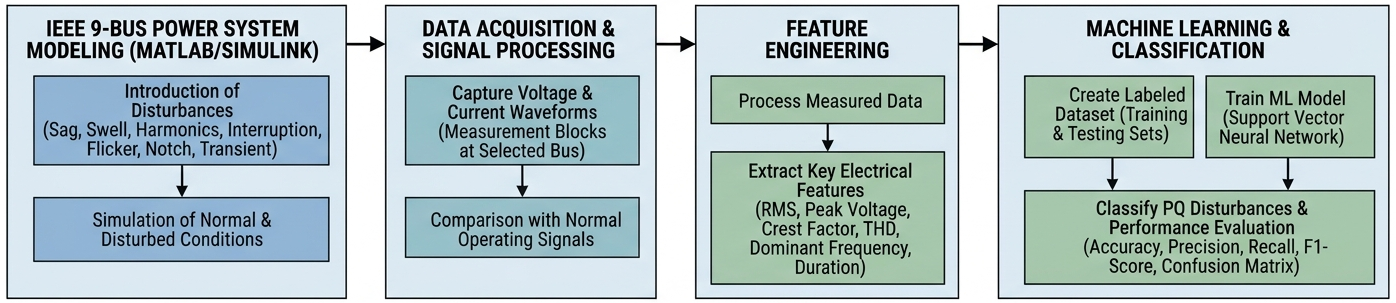
\includegraphics[width=0.95\textwidth]{block diagram_1.png}
    \caption{High-Level End-to-End System Architecture}
    \label{fig:sys_arch}
\end{figure}

The architecture consists of three principal modules:
\begin{enumerate}
    \item \textbf{Electromagnetic Simulation \& Signal Acquisition Module:} The WSCC 9-bus transmission model simulated in MATLAB/Simulink with controlled disturbance blocks generates continuous three-phase voltages ($V_{abc}$) and currents ($I_{abc}$) at Bus 5. Signals are acquired at 20 kHz and decimated to 5 kHz using an anti-aliasing Chebyshev lowpass filter.
    \item \textbf{DSP \& Feature Extraction Engine:} Continuous streams are sliced into 200 ms sliding observation windows (12 fundamental cycles at 60 Hz). The DSP engine extracts the canonical 32-dimensional feature contract comprising amplitude, signal quality, harmonic Goertzel magnitudes, and spectral moments.
    \item \textbf{Multi-Model Inference \& Visualization Module:} The extracted features and raw waveforms feed three model families: classical machine learning, raw waveform deep learning (1D CNN and TCN), and the multi-modal \textbf{HybridPQNet}. Results are served to an interactive research dashboard built on Streamlit.
\end{enumerate}

\section{Systematic Implementation Stages}
The methodology is executed across six structured engineering stages, depicted in Figures \ref{fig:step1_3} and \ref{fig:step4_6}.

\begin{figure}[H]
    \centering
    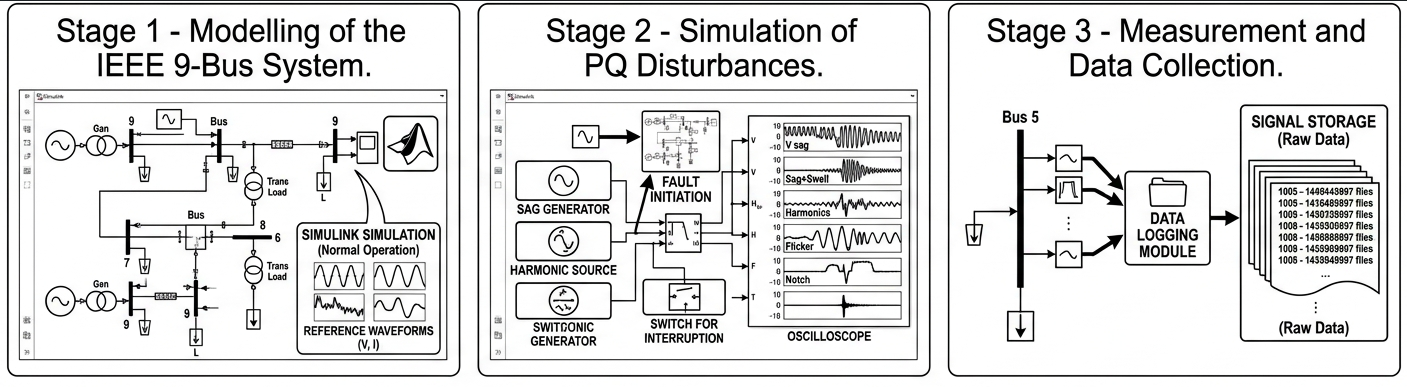
\includegraphics[width=0.95\textwidth]{step1_3.png}
    \caption{Power System Simulation, Disturbance Injection, and Raw Signal Measurement Workflow (Stages 1--3)}
    \label{fig:step1_3}
\end{figure}

\begin{figure}[H]
    \centering
    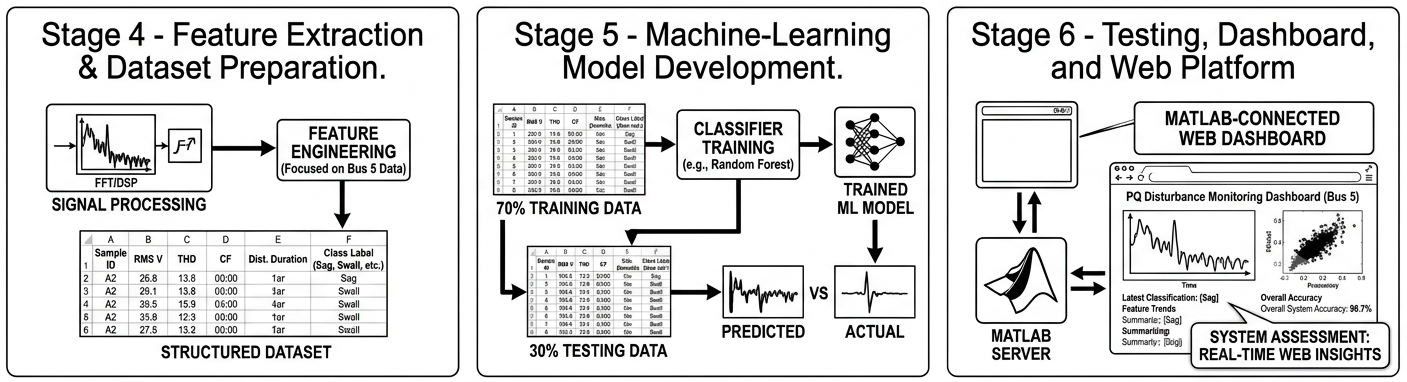
\includegraphics[width=0.95\textwidth]{step4_6.png}
    \caption{Digital Signal Processing, Model Benchmarking, and Evaluation Workflow (Stages 4--6)}
    \label{fig:step4_6}
\end{figure}

\subsection{Stage 1: Electrical Benchmark Modeling}
The Western System Coordinating Council (WSCC) 3-machine 9-bus benchmark represents a realistic 230 kV transmission network with three synchronous generating stations (Generator 1: 247.5 MVA, 16.5 kV; Generator 2: 192.0 MVA, 18.0 kV; Generator 3: 128.0 MVA, 13.8 kV) interconnected through step-up transformers and transmission lines to three major load centers at Buses 5, 6, and 8. The system is solved using the stiff numerical integrator \texttt{ode23tb} with a maximum step size capped strictly at $25\ \mu\text{s}$, guaranteeing numerical fidelity up to the 10 kHz Nyquist frequency.

\subsection{Stage 2: Disturbance Injection Mechanisms}
Disturbances are simulated physically within the circuit topology rather than superimposed as mathematical functions:
\begin{itemize}
    \item \textbf{Sag:} Shunt faults applied through timed three-phase fault breakers at Bus 4 with fault resistances $R_f \in [1.0, 30.0]\ \Omega$ and ground resistances $R_g \in [0.1, 5.0]\ \Omega$.
    \item \textbf{Swell:} Shunt three-phase capacitor bank energization ($Q_c \in [90, 150]\ \text{MVAR}$) at Bus 5 switched via circuit breakers.
    \item \textbf{Interruption:} Series breaker opening on transmission Line 4--5 isolating Bus 5.
    \item \textbf{Harmonics:} Controlled non-linear current injection spanning 3rd, 5th, 7th, 9th, and 11th harmonic orders.
    \item \textbf{Flicker:} Sub-band amplitude modulation ($f_m \in [3, 20]\text{ Hz}$, modulation depth $2\%\text{--}12\%$).
    \item \textbf{Notch:} Commutation notches created by periodic switching thyristor pairs (notch width $200\text{--}500\ \mu\text{s}$, 2 to 6 notches per cycle).
    \item \textbf{Transient:} High-frequency capacitor switching with damped RLC resonance ($f_{\text{osc}} \in [1.2, 2.2]\text{ kHz}$, damping time $\tau \in [25, 35]\text{ ms}$).
\end{itemize}

\subsection{Stage 3: Measurement and Noise Modeling}
Signals are observed at Bus 5 via Three-Phase V-I Measurement blocks:
\begin{equation}
v_{\text{meas}}(t) = Q_B\left(v_{\text{true}}(t) + n(t)\right)
\end{equation}
where $n(t)$ is zero-mean additive white Gaussian noise calibrated against nominal power ($P_{\text{nom}} = 0.3466\text{ pu}^2$, $\sigma = 0.001479\text{ pu}$ at 52 dB SNR), and $Q_B(\cdot)$ represents a bipolar symmetric quantizer with full-scale range $[-1.8\text{ pu}, +1.8\text{ pu}]$ at 12-bit ($\Delta = 8.789 \times 10^{-4}\text{ pu}$) or 14-bit ($\Delta = 2.197 \times 10^{-4}\text{ pu}$) resolution.

\subsection{Stage 4: Dual-Rate DSP and Feature Extraction}
Signals are sampled concurrently at 20 kHz (4,000 samples per 200 ms frame) for deep learning and decimated to 5 kHz (1,000 samples per frame) using a zero-phase 8th-order Chebyshev Type I lowpass filter ($f_c = 2.25\text{ kHz}$, passband ripple $0.05\text{ dB}$, stopband attenuation $>60\text{ dB}$). The canonical 32-feature contract is computed from the 5 kHz stream.

\subsection{Stage 5: Model Training and Multi-Modal Fusion}
Models are trained under strict partition isolation. Feature-based classical models are trained with \texttt{StandardScaler} fitted exclusively on training data. Deep learning models are trained using the Adam optimizer with cosine annealing learning rate schedules. \textbf{HybridPQNet} fuses the 64-dimensional feature vector from a 1D CNN waveform encoder with a 32-dimensional dense feature representation into a 96-dimensional shared embedding layer.

\subsection{Stage 6: Testing, Evaluation, and Failure Auditing}
Candidate models are evaluated across multi-class accuracy, balanced accuracy, Macro Precision, Macro Recall, and Macro F1 score. Furthermore, every simulated trajectory is validated against automated physical validation gates (IEEE Std 1159 voltage bounds, waveform continuity, and unbalance ratios).

\subsection{Physical Measurement and Signal-Conditioning Interface Context}
To establish the bridge between simulated transmission bus voltages and real-world edge hardware, this section details the analog signal-conditioning front-end architecture required for physical instrument acquisition. In physical electrical installations, high-voltage transmission lines ($230\text{ kV}$ nominal base, or $230\text{ V}_{\text{rms}}$ in laboratory prototypes) cannot be interfaced directly with sensitive digital signal processors or microcontroller ADCs. The front-end instrumentation encompasses four sequential conditioning stages:
\begin{enumerate}
    \item \textbf{Galvanic Sensing and Step-Down Attenuation:} Step-down potential transformers (PT) and precision non-inductive resistive dividers attenuate the transmission voltage down to instrumentation levels ($0\text{--}5\text{ V}$ peak-to-peak), providing high-voltage galvanic isolation.
    \item \textbf{Differential Amplification and Common-Mode Rejection:} A precision instrumentation operational amplifier stage provides high common-mode rejection ratio (CMRR $>90\text{ dB}$), rejecting ground-loop noise and high-voltage grid transients.
    \item \textbf{Active Anti-Aliasing Low-Pass Filtering:} A second-order active Butterworth low-pass filter ($f_c = 2.25\text{ kHz}$) suppresses out-of-band radio frequency interference and high-frequency switching harmonics, guaranteeing strict compliance with the Nyquist sampling theorem prior to digital conversion.
    \item \textbf{DC Level-Shifting and Overvoltage Clamping:} An active summing amplifier injects a stable $+1.65\text{ V}$ (or $+2.5\text{ V}$) reference bias, mapping bipolar sinusoidal AC voltages ($[-1.65\text{ V}, +1.65\text{ V}]$) into a unipolar $[0\text{ V}, 3.3\text{ V}]$ dynamic range suitable for embedded ADCs (such as ESP32, STM32, or external 14-bit ADCs), protected by high-speed Schottky clamping diodes against destructive spikes.
\end{enumerate}
While the present research focuses on high-fidelity numerical waveforms generated in MATLAB/Simulink with fixed-reference Gaussian sensor noise, this signal-conditioning topology defines the physical interface for future Phase 6 hardware-in-the-loop (HIL) testing.

\section{Standards Traceability and Project-Specific Classification Framework}
To establish a rigorous foundation for power quality disturbance monitoring, this project aligns its disturbance taxonomy, simulation parameters, and feature extraction with authoritative international standards, primarily \textbf{IEEE Std 1159-2019} \cite{ieee1159}, \textbf{IEEE Std 519-2022} \cite{ieee519}, and \textbf{IEEE Std 1453-2022} \cite{ieee1453}.

\subsection{Standards Taxonomy and Functional Governance}
The source document \textit{IEEE Standards.docx} articulates the distinct roles of the relevant IEEE standards:
\begin{enumerate}
    \item \textbf{IEEE Std 1159-2019 (Primary Taxonomy and Classification):} Provides the definitive classification of electromagnetic phenomena in electric power systems, establishing mathematical boundaries for short-duration voltage variations (sag, swell, interruption), transients, waveform distortion (harmonics, notch), and voltage fluctuations.
    \item \textbf{IEEE Std 519-2022 (Harmonic Control at the PCC):} Establishes harmonic voltage and current distortion limits specifically at the Point of Common Coupling (PCC) between utility systems and end-users. It serves as a regulatory standard for grid distortion limits rather than a universal multi-class classifier. Crucially, a heuristic threshold such as $\text{THD} > 5\%$ must not be treated as a standalone IEEE classification rule for general waveforms unless the specific PCC voltage tier and short-circuit ratio apply.
    \item \textbf{IEEE Std 1453-2022 (Voltage Fluctuations and Flicker):} Defines measurement protocols and limits for voltage fluctuations inducing lamp flicker, mandating the calculation of short-term flicker severity ($P_{st}$) over 10-minute intervals and long-term severity ($P_{lt}$) over 2-hour intervals using an IEC 61000-4-15 flickermeter \cite{iec61000}.
    \item \textbf{IEEE Std 1159.3-2025 (Data Interchange / PQDIF):} Specifies the standardized binary file format (Power Quality Data Interchange Format) and metadata schema for exchanging waveform and event records, governing data transport rather than classification logic \cite{ieee1159_3}.
\end{enumerate}

\subsection{Frequency Adaptation: 50 Hz Standards Examples vs. 60 Hz Benchmark Implementation}
The reference standards document (\textit{IEEE Standards.docx}) utilizes 50 Hz illustrative examples, reflecting European and Indian utility operating frequencies. In this project, however, the benchmark system is the Western System Coordinating Council (WSCC) IEEE 9-bus grid, which operates at a nominal base frequency of \textbf{60.0 Hz}. 

Directly copying 50 Hz cycle-to-millisecond conversions into a 60 Hz simulation benchmark introduces severe timing errors. At 50 Hz, one electrical cycle spans $T_{50} = 20.0\text{ ms}$, meaning a 200 ms observation window encompasses exactly 10 cycles. At 60 Hz, one cycle spans $T_{60} = 1/60 \approx 16.667\text{ ms}$, meaning the exact same 200 ms window encompasses \textbf{exactly 12 fundamental cycles}:
\begin{equation}
N_{\text{cycles}} = \frac{T_{\text{window}}}{T_{60}} = \frac{0.200\text{ s}}{0.016667\text{ s}} = 12.0\text{ cycles}
\end{equation}
Table \ref{tab:freq_mapping} provides the precise mathematical conversion between 50 Hz standard illustrative benchmarks and the 60 Hz parameters implemented in this project.

\begin{table}[H]
\centering
\caption{Cycle and Duration Mapping: 50 Hz Standard Examples vs. Implemented 60 Hz Benchmark}
\label{tab:freq_mapping}
\small
\begin{tabularx}{\textwidth}{lXX}
\toprule
\textbf{Parameter / Event Category} & \textbf{50 Hz Standards Example (\textit{IEEE Standards.docx})} & \textbf{60 Hz Benchmark Implementation (This Project)} \\
\midrule
Fundamental Frequency ($f_0$) & $50.0\text{ Hz}$ & $\mathbf{60.0\text{ Hz}}$ \\
Cycle Duration ($T_0 = 1/f_0$) & $20.0\text{ ms}$ & $\mathbf{16.667\text{ ms}}$ \\
200 ms Observation Window ($T_w$) & $10.0\text{ cycles}$ & $\mathbf{12.0\text{ cycles}}$ \\
Instantaneous Sag / Swell ($0.5\text{--}30\text{ cycles}$) & $10.0\text{ ms to }600.0\text{ ms}$ & $\mathbf{8.33\text{ ms to }500.0\text{ ms}}$ \\
Momentary Interruption ($0.5\text{ cycle to }3.0\text{ s}$) & $10.0\text{ ms to }3.0\text{ s}$ & $\mathbf{8.33\text{ ms to }3.0\text{ s}}$ \\
Typical Simulated Disturbance Duration & $2\text{--}10\text{ cycles } (40\text{--}200\text{ ms})$ & $\mathbf{5\text{--}6\text{ cycles } (83.3\text{--}100.0\text{ ms})}$ \\
Harmonic Order H2 (2nd Harmonic) & $100.0\text{ Hz}$ & $\mathbf{120.0\text{ Hz}}$ \\
Harmonic Order H3 (3rd Harmonic) & $150.0\text{ Hz}$ & $\mathbf{180.0\text{ Hz}}$ \\
Harmonic Order H5 (5th Harmonic) & $250.0\text{ Hz}$ & $\mathbf{300.0\text{ Hz}}$ \\
Harmonic Order H7 (7th Harmonic) & $350.0\text{ Hz}$ & $\mathbf{420.0\text{ Hz}}$ \\
Harmonic Order H9 (9th Harmonic) & $450.0\text{ Hz}$ & $\mathbf{540.0\text{ Hz}}$ \\
Harmonic Order H11 (11th Harmonic) & $550.0\text{ Hz}$ & $\mathbf{660.0\text{ Hz}}$ \\
\bottomrule
\end{tabularx}
\end{table}

\subsection{Project-Specific Disturbance Classification Matrix}
Table \ref{tab:classification_matrix} incorporates the complete power-quality disturbance classification table from \textit{IEEE Standards.docx}, rigorously adapted and reconciled against the actual MATLAB/Simulink models, scenario matrices, DSP feature extraction code, and evaluation artifacts of this project.

\begin{table}[H]
\centering
\caption{Power Quality Disturbance Standards Criteria vs. Implemented Project Specifications}
\label{tab:classification_matrix}
\tiny
\setlength{\tabcolsep}{3pt}
\renewcommand{\arraystretch}{1.2}
\begin{tabularx}{\textwidth}{p{1.7cm}p{1.6cm}p{2.5cm}p{2.7cm}p{2.7cm}p{2.4cm}}
\toprule
\textbf{Disturbance Class} & \textbf{Applicable Standard / Ref.} & \textbf{Standard-Derived Classification Criteria} & \textbf{Project Simulation \& Generation Method} & \textbf{Signal-Processing \& Analysis Method} & \textbf{Project Implementation Status \& Scope} \\
\midrule
\textbf{Normal Operation} & IEEE Std 1159-2019 framework & Nominal steady-state sinusoid; $0.90 \le V_{\text{rms}} \le 1.10\text{ pu}$; no qualifying PQ disturbance. & Unperturbed WSCC 9-bus power flow across 10 generator/load dispatches; $V_{\text{rms}} \in [0.555, 0.635]\text{ pu}$. & True RMS calculation, zero-crossing frequency tracking, Goertzel THD, and 3-phase unbalance check. & \textbf{Fully Implemented.} 1,120 frames in baseline, 576 frames in Phase 5C. Verified $\text{THD} < 0.09\%$. \\
\addlinespace
\textbf{Voltage Sag} & IEEE Std 1159-2019 & Temporary reduction in RMS voltage: $0.10 \le V_{\text{rms}} < 0.90\text{ pu}$; instantaneous: $0.5\text{--}30\text{ cycles}$ ($8.33\text{--}500\text{ ms}$ at 60 Hz). & Shunt fault at Bus 4 via \texttt{PQD\_Fault\_Sag} ($R_f \in [1, 30]\ \Omega$, $R_g \in [0.1, 5]\ \Omega$); duration $80\text{--}100\text{ ms}$ ($\approx 5\text{--}6\text{ cycles}$). & Sliding 200 ms window RMS ($V_{\text{rms}}$), duration ($T_{\text{dur}}$), and crest factor ($CF = V_{\text{peak}} / V_{\text{rms}}$). & \textbf{Fully Implemented.} 18 continuous trajectories, 576 frames. Validated residual $V_{\text{rms}} \in [0.15, 0.85]\text{ pu}$. \\
\addlinespace
\textbf{Voltage Swell} & IEEE Std 1159-2019 & Temporary increase in RMS voltage: $1.10 < V_{\text{rms}} \le 1.80\text{ pu}$ instantaneous ($0.5\text{--}30\text{ cycles}$); momentary: $1.10\text{--}1.40\text{ pu}$ ($30\text{ cycles to }3\text{ s}$). & Shunt capacitor energization at Bus 5 via \texttt{PQD\_Breaker\_Swell} ($Q_c = 90\text{--}150\text{ MVAR}$); duration $80\text{--}100\text{ ms}$. & Windowed RMS, duration, crest factor, and post-clearing transient overshoot tracking. & \textbf{Fully Implemented.} 576 frames. 10 runs flagged in registry due to snubber trapped-charge overvoltage. \\
\addlinespace
\textbf{Voltage Interruption} & IEEE Std 1159-2019 & Supply collapse: $V_{\text{rms}} < 0.10\text{ pu}$; momentary: $0.5\text{ cycle to }3\text{ s}$ ($8.33\text{ ms to }3.0\text{ s}$ at 60 Hz); temporary: $>3\text{ s to }1\text{ min}$. & Series circuit breaker opening on Line 4--5 via \texttt{PQD\_Breaker\_Interruption}; duration $80\text{--}100\text{ ms}$. & Windowed RMS $<0.1\text{ pu}$ duration tracking and orthogonal SNR projection. & \textbf{Fully Implemented.} 576 frames. Bus 5 voltage collapses below $0.05\text{ pu}$ during series isolation. \\
\addlinespace
\textbf{Harmonics} & IEEE Std 1159-2019 + IEEE Std 519-2022 & Waveform distortion with integer-multiple components. Note: $\text{THD} > 5\%$ is a PCC limit in IEEE 519, not a general waveform classifier. & Controlled non-linear load current injection at Bus 5 spanning odd orders: H3 (180 Hz), H5 (300 Hz), H7 (420 Hz), H9 (540 Hz), H11 (660 Hz). & Goertzel algorithm for individual harmonic bins H1--H11, odd harmonic ratios ($H_n/H_1$), total harmonic energy, and spectral centroid. & \textbf{Fully Implemented.} 576 frames. Model evaluates Goertzel harmonic features; $\text{THD} \in [5.2\%, 25.0\%]$. \\
\addlinespace
\textbf{Oscillatory Transient} & IEEE Std 1159-2019 (Category 1.2.1) & Low-frequency oscillatory transient: spectral content $<5\text{ kHz}$; duration $0.3\text{--}50\text{ ms}$; peak magnitude $0\text{--}4\text{ pu}$. & High-frequency capacitor switching with damped RLC resonance at Bus 5 ($f_{\text{osc}} \in [1.2, 2.2]\text{ kHz}$, damping time $\tau \in [25, 35]\text{ ms}$). & Orthogonal projection SNR (primary discriminator), crest factor, duration, spectral flatness, and 20 kHz raw waveform convolutions. & \textbf{Fully Implemented.} 576 frames. 5 kHz decimation imposes 2.5 kHz Nyquist limit; 20 kHz branch captures full transient profile. \\
\addlinespace
\textbf{Voltage Flicker} & IEEE Std 1159-2019 + IEEE Std 1453-2022 & Voltage fluctuation with modulation frequency $<25\text{ Hz}$. True assessment requires IEC 61000-4-15 flickermeter ($P_{st}/P_{lt}$). & Low-frequency sinusoidal sub-band amplitude modulation ($f_m \in [3.0, 20.0]\text{ Hz}$, modulation depth $2.0\%\text{--}12.0\%$). & Sub-band envelope extraction, sub-sample zero-crossing tracking (\texttt{system\_freq}), and spectral entropy. & \textbf{Simplified ML Proxy Implemented.} 200 ms frame serves as an ML classification proxy; full flickermeter assessment is demarcated as future scope. \\
\addlinespace
\textbf{Commutation\newline Notch} & IEEE Std 1159-2019 & Periodic sub-cycle voltage depressions due to converter commutation; no single universal IEEE numerical threshold. & Periodic sub-cycle voltage notch injection via timed switching thyristors (width $200\text{--}500\ \mu\text{s}$, 2 to 6 notches per cycle). & Time-domain difference error against baseline sinusoid, crest factor, and 20 kHz raw waveform convolutional feature extraction. & \textbf{Fully Implemented.} 576 frames. 20 kHz sampling yields 8 discrete samples per $400\ \mu\text{s}$ notch vs. only 2 samples at 5 kHz. \\
\bottomrule
\end{tabularx}
\end{table}

\subsection{Connecting the Standards Criteria to Experimental Results}
The standards-derived criteria formalised in Table \ref{tab:classification_matrix} govern every component of the experimental pipeline:
\begin{enumerate}
    \item \textbf{Simulink Disturbance Generation:} The physical injection mechanisms modeled in \texttt{IEEE\_9bus\_PQD\_DISTURBANCES.slx} (Section \ref{sec:simulink_clean}) are strictly calibrated against the IEEE Std 1159 magnitude boundaries ($0.1\text{--}0.9\text{ pu}$ for Sag, $1.1\text{--}1.8\text{ pu}$ for Swell, $<0.1\text{ pu}$ for Interruption).
    \item \textbf{Signal Acquisition at Bus 5:} Because IEEE Std 1159 identifies low-frequency oscillatory transients up to 5 kHz and commutation notches down to $200\ \mu\text{s}$, the project implements a dual-rate acquisition architecture. The 5 kHz branch satisfies Nyquist criteria for fundamental harmonics up to the 11th order (660 Hz), while the 20 kHz high-resolution branch resolves high-frequency capacitor ringing (1.2--2.2 kHz) and sub-cycle notch slopes.
    \item \textbf{Feature Extraction and Disturbance Labels:} The canonical 32-feature contract (Table \ref{tab:32_features}) directly translates standard phenomena into numerical descriptors: \texttt{rms\_voltage} and \texttt{duration} govern short-duration variations; \texttt{h1} through \texttt{h11} and \texttt{thd} govern harmonic distortion; \texttt{snr} and \texttt{crest\_factor} isolate oscillatory transients; and \texttt{system\_freq} captures flicker modulation.
    \item \textbf{Dataset Validation \& Failure Auditing:} The automated physical validation suite checks each simulated trajectory against the bounds in Table \ref{tab:classification_matrix}. The 26 flagged trajectories (Section \ref{sec:dataset_freeze}) illustrate where standard-derived assumptions interact with physical grid behavior---such as capacitive breaker snubber trapped charges and power-flow voltage shifts.
    \item \textbf{Machine-Learning Evaluation:} Connecting these physical descriptors to machine-learning models explains why the multi-modal \textbf{HybridPQNet} (Section \ref{sec:hybrid_breakthrough}) achieves 100.00\% classification accuracy: the 1D CNN branch resolves sub-cycle notch morphology and transient phase coupling, while the engineered feature branch provides exact mathematical integrals for true RMS and Goertzel harmonic ratios.
\end{enumerate}

% =========================================================================
% CHAPTER 4: IEEE 9-BUS BENCHMARK AND SIMULINK DEMONSTRATION
% =========================================================================
\chapter{IEEE 9-Bus Benchmark Model and Simulink Demonstration}

\section{WSCC IEEE 9-Bus Model Structure}
The Western System Coordinating Council (WSCC) 3-machine 9-bus benchmark system is widely acknowledged as the international standard for power system transient stability and power quality research. The network consists of:
\begin{itemize}
    \item 3 Generating units with individual excitation and governor systems (Gen 1: 247.5 MVA, 16.5 kV; Gen 2: 192.0 MVA, 18.0 kV; Gen 3: 128.0 MVA, 13.8 kV);
    \item 3 Two-winding step-up transformers (16.5/230 kV, 18/230 kV, 13.8/230 kV);
    \item 6 High-voltage 230 kV transmission lines (Lines 4--5, 5--7, 7--8, 8--9, 6--9, 4--6);
    \item 3 Main load buses (Bus 5: $125\text{ MW} + j50\text{ MVAR}$; Bus 6: $90\text{ MW} + j30\text{ MVAR}$; Bus 8: $100\text{ MW} + j35\text{ MVAR}$).
\end{itemize}
Figure \ref{fig:ieee9bus_schematic} displays the authoritative single-line diagram of the WSCC 9-bus benchmark network exported directly from the reference system specification (\textit{original 9 bus.pdf}), showing the spatial topology connecting the generating stations, step-up transformers, and load centers, with Bus 5 serving as the primary power quality observation bus.

\begin{figure}[H]
    \centering
    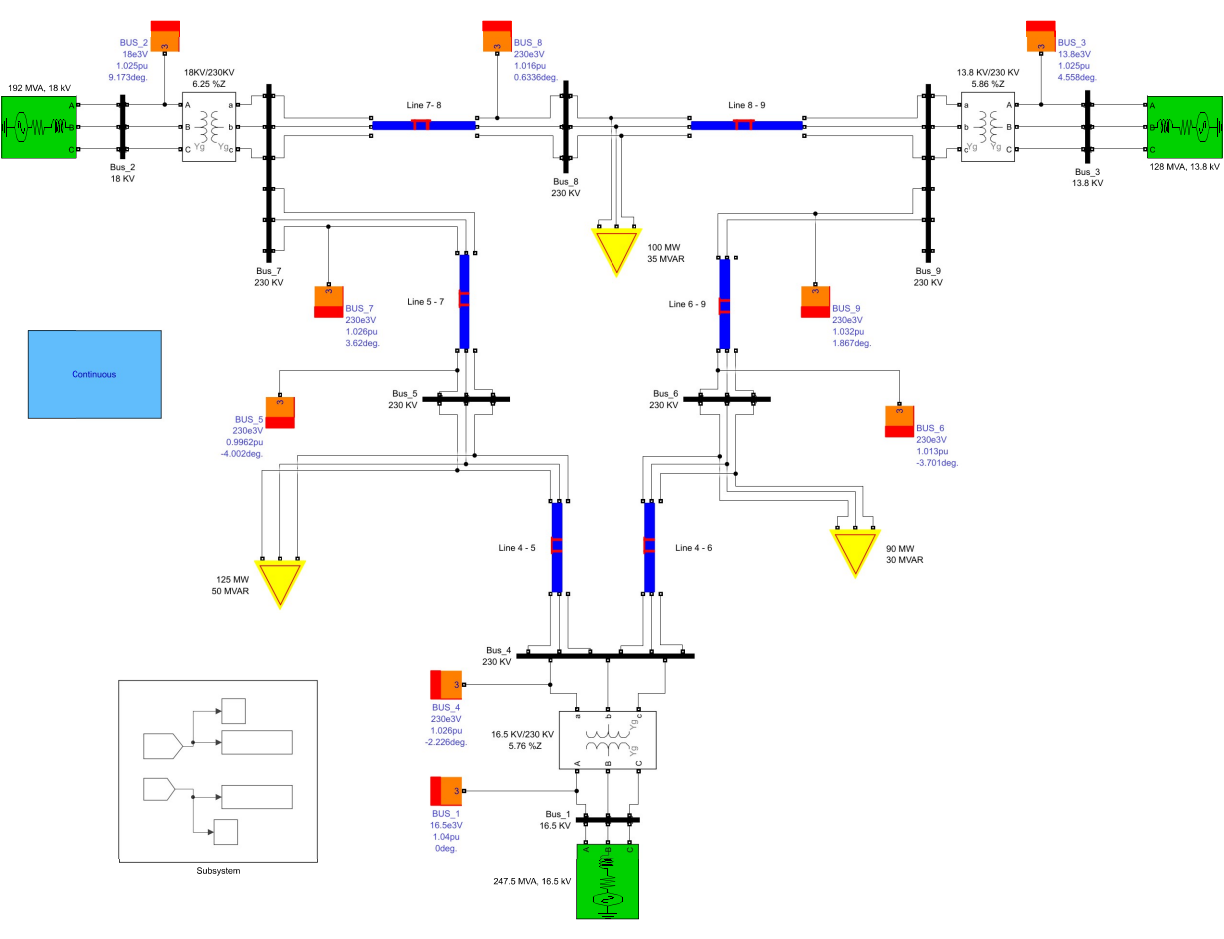
\includegraphics[width=0.85\textwidth]{original_9bus_baseline_model.png}
    \caption{WSCC IEEE 9-bus 3-machine benchmark electrical transmission single-line diagram, depicting generators at Buses 1, 2, and 3, step-up transformers, 230 kV transmission lines, and the observation load bus at Bus 5 (extracted directly from \textit{original 9 bus.pdf}).}
    \label{fig:ieee9bus_schematic}
\end{figure}

\subsection{Disturbance-Injection Topology and Network Modifications}
To inject physical power quality disturbances into the benchmark grid, controlled switching and fault blocks are embedded into the transmission branches. Figure \ref{fig:circuit1_model} illustrates the circuit diagram exported from the project reference documentation (\textit{circuit 1.pdf}). A timed three-phase fault block (\texttt{Fault for Voltage Sag}) and series circuit breakers (\texttt{Breaker for Interruption} and \texttt{Breaker 2 for Interruption}) are placed on Line 5--7 and Line 4--5, enabling precise temporal control over fault inception, ground resistance, and transmission line isolation.

\begin{figure}[H]
    \centering
    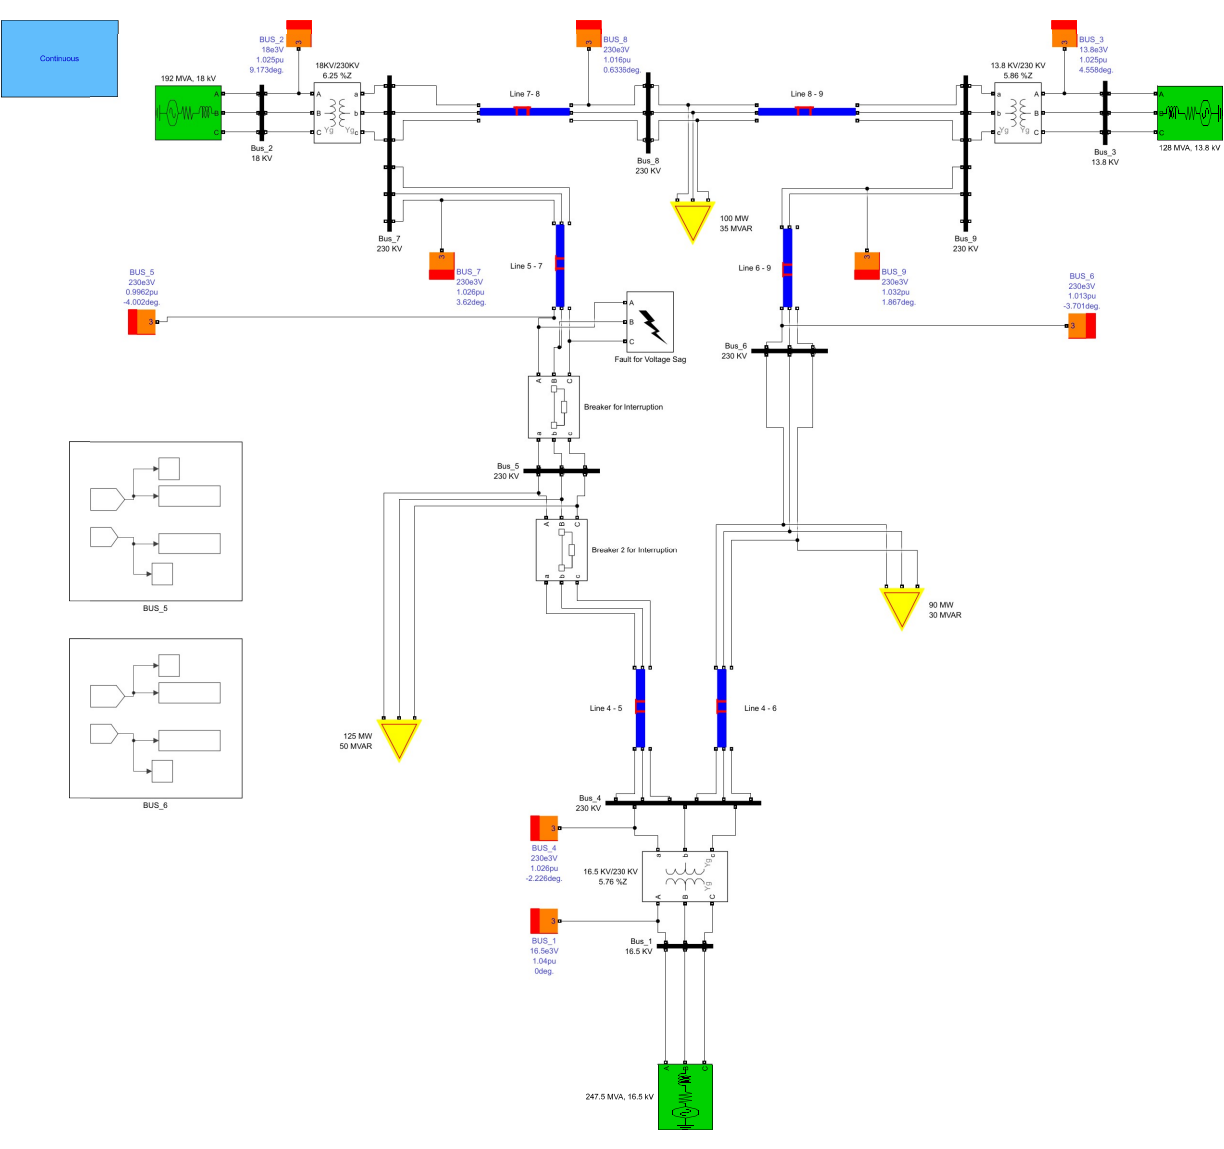
\includegraphics[width=0.85\textwidth]{circuit1_fault_injection_model.png}
    \caption{Simulink IEEE 9-bus circuit diagram showing the physical placement of disturbance-injection blocks: three-phase fault block on Line 5--7 and series interruption breakers (extracted directly from \textit{circuit 1.pdf}).}
    \label{fig:circuit1_model}
\end{figure}

\subsection{Working Disturbance Model vs. Protected Pristine Reference}
In this project, two distinct Simulink models are maintained to guarantee strict research integrity:
\begin{enumerate}
    \item \textbf{Working Disturbance Model (\texttt{IEEE\_9bus/IEEE\_9bus\_PQD\_DISTURBANCES.slx}):} Contains all active disturbance injection blocks, programmable breakers, fault blocks, and observation interfaces (\texttt{PQD\_Vabc} and \texttt{PQD\_Iabc}). This model is utilized for all simulation runs, scenario injections, and dataset generations.
    \item \textbf{Protected Pristine Reference Model (\texttt{IEEE\_9bus/IEEE\_9bus\_PQD\_HIL\_R2025a.slx}):} Serves as the byte-for-byte untouched baseline reference. Its cryptographic integrity is verified via SHA-256:
    \begin{equation}
    \text{SHA-256: } \texttt{5D833D8FDC5086B7BEC437A30A7829B4EA6D1B9BEFA93DF75E7CA0631BEB084D}
    \end{equation}
    This reference model remains completely unmodified throughout all research phases.
\end{enumerate}

\section{Simulink Model Configurations: Clean Baseline vs. Fault-Injected Benchmark}
Figure \ref{fig:simulink_clean} displays the working Simulink model in its clean, baseline, no-fault operational state. In this baseline configuration, all fault blocks (\texttt{PQD\_Fault\_Sag}) have their fault phases disabled (\texttt{FaultA = off}, \texttt{FaultB = off}, \texttt{FaultC = off}, \texttt{SwitchTimes = [999 1000]}), swell capacitor breakers (\texttt{PQD\_Breaker\_Swell}) are held in the open state, and harmonic/flicker/notch enable switches are deactivated. The diagram exhibits no temporary red fault overlays or selection artifacts.

In contrast, Figure \ref{fig:simulink_fault_annotated} illustrates the working disturbance model (\texttt{IEEE\_9bus\_PQD\_DISTURBANCES.slx}) in its active simulation state, featuring the visible red/orange highlighting around the disturbance injection subsystems (such as the Bus 4 shunt fault breaker, Bus 5 capacitor energization bank, non-linear harmonic load, and line interruption switch) and the Bus 5 measurement interfaces. Comparing Figures \ref{fig:simulink_clean} and \ref{fig:simulink_fault_annotated} clearly distinguishes the pristine baseline network from the fault-instrumented research benchmark.

\begin{figure}[H]
    \centering
    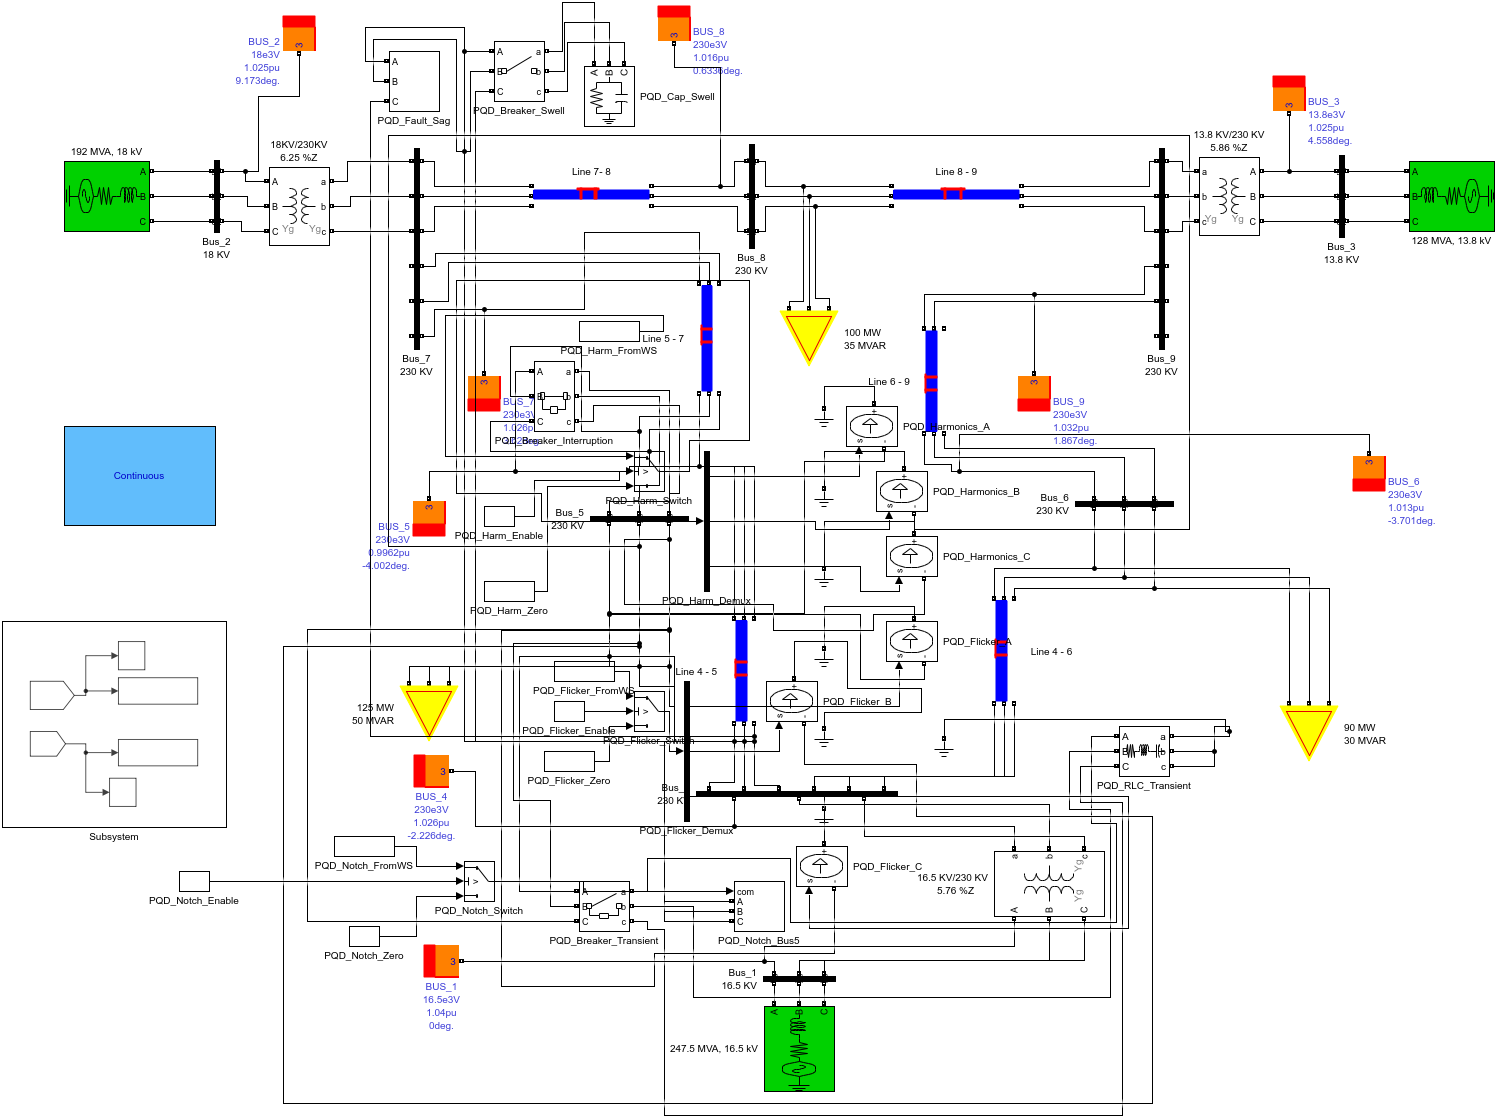
\includegraphics[width=0.98\textwidth]{simulink_model_clean.png}
    \caption{IEEE 9-bus power system model in the baseline, no-disturbance configuration (exported directly from MATLAB/Simulink R2025a without fault-highlighting overlays).}
    \label{fig:simulink_clean}
\end{figure}

\begin{figure}[H]
    \centering
    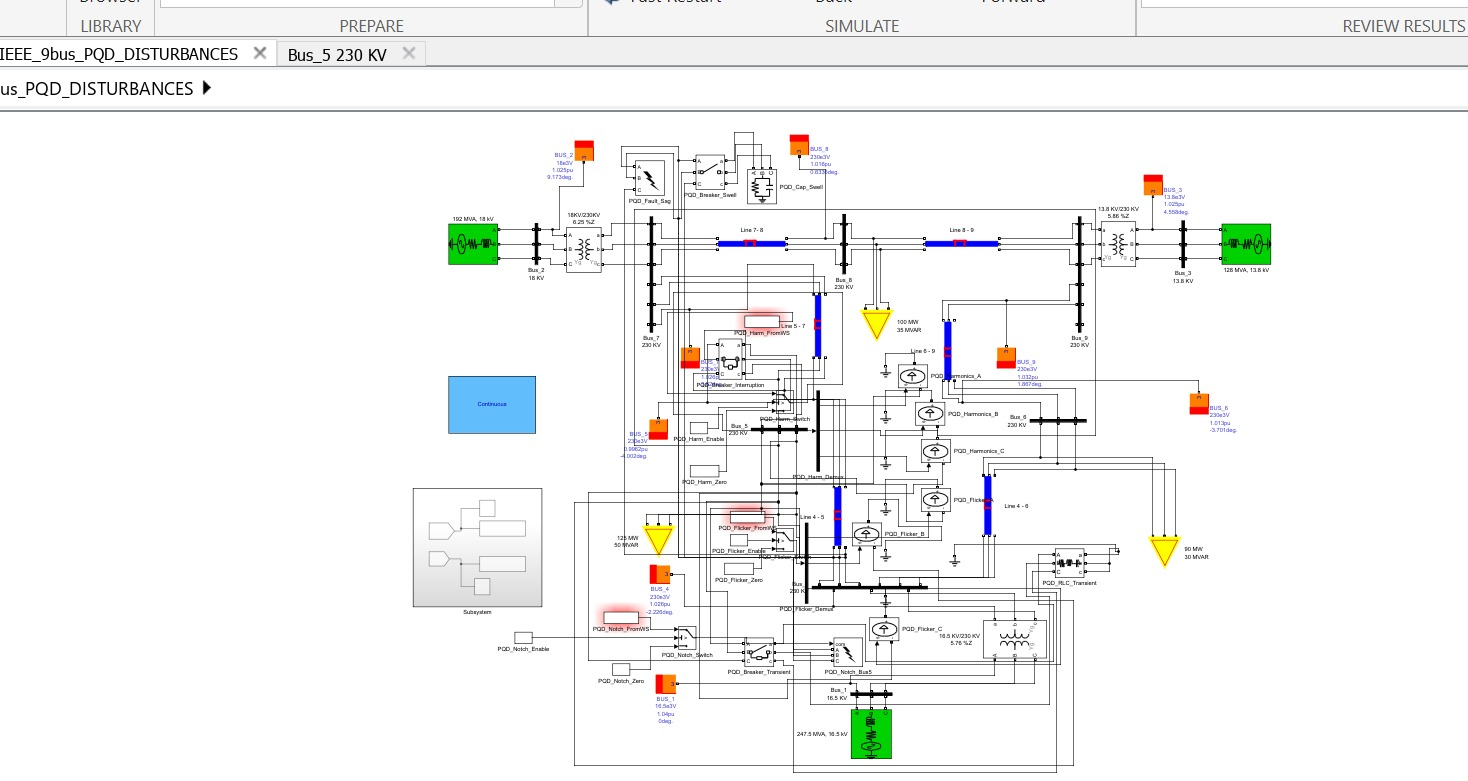
\includegraphics[width=0.98\textwidth]{simulink_fault_annotated.png}
    \caption{Working disturbance model (\texttt{IEEE\_9bus\_PQD\_DISTURBANCES.slx}) in the active simulation configuration, showing the red/orange highlighted disturbance-injection blocks and Bus 5 measurement instrumentation.}
    \label{fig:simulink_fault_annotated}
\end{figure}

\section{Dedicated MATLAB Sag and Swell Demonstration Guide}
To provide students, examiners, and researchers with an exact, reproducible procedure for demonstrating Voltage Sag and Voltage Swell in MATLAB/Simulink, this section outlines the physical mechanism, simulation execution, and waveform analysis.

\subsection{Physical Mechanisms of Sag and Swell Injection}
\begin{itemize}
    \item \textbf{Voltage Sag Mechanism:} A controlled three-phase shunt fault is applied at Bus 4 via \texttt{PQD\_Fault\_Sag}. When the fault breaker closes at $t = 0.12\text{ s}$, fault current surges through the small fault resistance ($R_f = 5.0\ \Omega$), collapsing the potential at Bus 4. Because Bus 5 is connected directly to Bus 4 via transmission Line 4--5, the voltage at Bus 5 sags to approximately $0.45\text{ pu}$ (a 55\% voltage reduction). At $t = 0.2033\text{ s}$ (duration: $\approx 5$ cycles), the breaker opens, clearing the fault, and system voltage recovers to nominal steady state.
    \item \textbf{Voltage Swell Mechanism:} A three-phase shunt capacitor bank ($Q_c = 120\text{ MVAR}$) located at Bus 5 is switched into service via \texttt{PQD\_Breaker\_Swell} at $t = 0.12\text{ s}$. The injection of large reactive power raises the local transmission bus voltage to approximately $1.15\text{--}1.29\text{ pu}$. At $t = 0.20\text{ s}$, the breaker opens at the current zero-crossing, returning the system to nominal voltage.
\end{itemize}

\subsection{Step-by-Step Practical MATLAB Demonstration Commands}
Users can execute the demonstrations using the copy-paste MATLAB scripts below, which are directly grounded in the Phase 5C continuous recordings in \texttt{data/ieee9bus\_60hz\_phase5c/raw/}:

\subsubsection{Option A: Inspecting and Visualizing Recorded Authoritative Trajectories}
Listing \ref{lst:matlab_demo} provides the complete verification, loading, metadata parsing, and four-panel plotting script for the Phase 5C Sag and Swell recordings:

\begin{lstlisting}[language=Matlab, caption={MATLAB script to verify, load, and plot Phase 5C Sag and Swell recordings}, label={lst:matlab_demo}]
% =========================================================================
% Practical MATLAB Script: Verify, Inspect, and Plot Phase 5C Recordings
% Grounded in data/ieee9bus_60hz_phase5c/raw/ and sc metadata contract
% =========================================================================

% 1. Set repository root directory
repo_root = 'D:\my study\Project\power-quality-detector-and-classifier';
if ~exist(repo_root, 'dir')
    error('Project repository directory not found: %s', repo_root);
end
cd(repo_root);

% 2. Define authoritative Sag and Swell recording paths
sag_file = fullfile(repo_root, 'data', 'ieee9bus_60hz_phase5c', 'raw', ...
    'P5B2_SAG_0091_abc_c01_mil.mat');
swe_file = fullfile(repo_root, 'data', 'ieee9bus_60hz_phase5c', 'raw', ...
    'P5B2_SWE_0109_abc_c01_mil.mat');

% Verify file existence before loading
if ~exist(sag_file, 'file') || ~exist(swe_file, 'file')
    error('Target MAT recording files not found in Phase 5C directory.');
end

% 3. Load recordings into MATLAB workspace
sag_data = load(sag_file);
swe_data = load(swe_file);

% 4. Inspect metadata from sc structure
fprintf('=== SAG RECORDING METADATA ===\n');
fprintf('Trajectory ID: %s\n', sag_data.sc.trajectory_id);
fprintf('Disturbance Class: %s\n', sag_data.sc.class);
fprintf('Operating Condition: %s\n', sag_data.sc.operating_condition_name);
fprintf('Sampling Rates: %d Hz (high-res), %d Hz (decimated)\n', ...
    sag_data.sc.sampling_rates_hz(1), sag_data.sc.sampling_rates_hz(2));
fprintf('Simulation Duration: %.2f s (%d continuous samples at 20 kHz)\n', ...
    sag_data.sc.simulation_duration_s, size(sag_data.V_cont_20k, 1));
fprintf('Disturbance Duration: %d ms, Onset Range: [%d, %d] ms\n\n', ...
    sag_data.sc.parameters.duration_ms, ...
    sag_data.sc.parameters.onset_range_ms(1), ...
    sag_data.sc.parameters.onset_range_ms(2));

fprintf('=== SWELL RECORDING METADATA ===\n');
fprintf('Trajectory ID: %s\n', swe_data.sc.trajectory_id);
fprintf('Disturbance Class: %s\n', swe_data.sc.class);
fprintf('Capacitive Power: %d MVAR\n', swe_data.sc.parameters.capacitive_power_mvar);
fprintf('Disturbance Duration: %d ms\n\n', swe_data.sc.parameters.duration_ms);

% 5. Data integrity check: NaN, Inf, and dimensions
assert(~any(isnan(sag_data.V_cont_20k(:))), 'NaN detected in Sag voltage!');
assert(~any(isinf(sag_data.V_cont_20k(:))), 'Inf detected in Sag voltage!');
assert(isequal(size(sag_data.V_cont_20k), [7601, 3]), 'Unexpected dimensions!');
fprintf('Integrity Check: PASSED (7,601 continuous points, zero NaN/Inf).\n');

% 6. Extract time vector and continuous waveforms (in per-unit [pu])
t_ms = sag_data.t_grid_20k * 1000.0; % Convert time from seconds to milliseconds
V_sag = sag_data.V_cont_20k;         % [7601 x 3] 3-phase voltage in pu
I_sag = sag_data.I_cont_20k;         % [7601 x 3] 3-phase current in pu
V_swe = swe_data.V_cont_20k;         % [7601 x 3] 3-phase voltage in pu
I_swe = swe_data.I_cont_20k;         % [7601 x 3] 3-phase current in pu

% 7. Plot Four-Panel Demonstration Figure
fig = figure('Name', 'IEEE 9-Bus Sag & Swell Demonstration (Phase 5C)', ...
    'Color', 'w', 'Position', [100, 100, 1000, 700]);

% Panel 1: Voltage Sag (Bus 5)
subplot(2,2,1);
plot(t_ms, V_sag, 'LineWidth', 1.1);
hold on;
xline(sag_data.sc.parameters.onset_range_ms(1), '--r', 'Onset Window');
xline(sag_data.sc.parameters.onset_range_ms(1) + sag_data.sc.parameters.duration_ms, ...
    '--k', 'Clearing');
hold off;
title(sprintf('Voltage Sag: %s (V_{abc})', sag_data.sc.trajectory_id), 'Interpreter', 'none');
ylabel('Voltage (pu)'); grid on; ylim([-1.5, 1.5]);
legend('Phase A', 'Phase B', 'Phase C', 'Location', 'northeast');

% Panel 2: Voltage Sag Current (Bus 5)
subplot(2,2,2);
plot(t_ms, I_sag, 'LineWidth', 1.1);
title('Voltage Sag: Fault Current Surge (I_{abc})');
ylabel('Current (pu)'); grid on; ylim([-2.0, 2.0]);
legend('Phase A', 'Phase B', 'Phase C', 'Location', 'northeast');

% Panel 3: Voltage Swell (Bus 5)
subplot(2,2,3);
plot(t_ms, V_swe, 'LineWidth', 1.1);
hold on;
xline(swe_data.sc.parameters.onset_range_ms(1), '--r', 'Capacitor ON');
xline(swe_data.sc.parameters.onset_range_ms(1) + swe_data.sc.parameters.duration_ms, ...
    '--k', 'Breaker Open');
hold off;
title(sprintf('Voltage Swell: %s (V_{abc})', swe_data.sc.trajectory_id), 'Interpreter', 'none');
xlabel('Time (ms)'); ylabel('Voltage (pu)'); grid on; ylim([-3.8, 3.8]);

% Panel 4: Voltage Swell Current (Bus 5)
subplot(2,2,4);
plot(t_ms, I_swe, 'LineWidth', 1.1);
title('Voltage Swell: Reactive Current (I_{abc})');
xlabel('Time (ms)'); ylabel('Current (pu)'); grid on; ylim([-4.5, 4.5]);

% 8. Export figure for documentation
exportgraphics(fig, 'doc/final_year_report_A/matlab_sag_swell_demo.png', 'Resolution', 300);
fprintf('Demonstration complete. Figure exported successfully.\n');
\end{lstlisting}

\subsubsection{Option B: Executing a Targeted Single Disturbance Simulation}
To execute a targeted single simulation without triggering the entire 144-trajectory batch, users invoke \texttt{run\_phase5c\_bulk\_simulation} with the specific trajectory identifier:

\begin{lstlisting}[language=Matlab, caption={MATLAB script to execute targeted single disturbance simulation}]
% =========================================================================
% Practical MATLAB Script: Execute Targeted Disturbance Simulation
% Runs scripts/run_phase5c_bulk_simulation.m for a specific trajectory
% =========================================================================

repo_root = 'D:\my study\Project\power-quality-detector-and-classifier';
cd(repo_root);
addpath(fullfile(repo_root, 'scripts'));
addpath(fullfile(repo_root, 'IEEE_9bus'));

% Target a single trajectory ID from scenarios/phase5b2_simulation_matrix.json
target_id = {'P5B2_SAG_0091_abc_c01_mil'};

fprintf('Launching targeted simulation for trajectory: %s\n', target_id{1});
run_phase5c_bulk_simulation(target_id);

fprintf('Simulation complete. Output saved to data/ieee9bus_60hz_phase5c/raw/\n');
\end{lstlisting}

\noindent
\textbf{Understanding Generation vs. Verification Execution:} When \texttt{run\_phase5c\_bulk\_simulation} is called with no arguments, it processes the 144 core trajectories specified in \texttt{scenarios/phase5b2\_simulation\_matrix.json}. Before running any Simulink model, the script checks whether \texttt{data/ieee9bus\_60hz\_phase5c/raw/<trajectory\_id>.mat} already exists with a valid 7,601-point continuous waveform. If it exists, the runner skips re-simulation to prevent overwriting verified data. In a recent audit, this verification mechanism evaluated all 144 files in 2.09 seconds, reporting \textbf{144 skipped, 0 newly simulated, and 0 failures}, confirming that all trajectories had been previously simulated and stored.

\subsection{Waveform Analysis: Voltage and Current Dynamics}
Figures \ref{fig:sag_wf} and \ref{fig:swell_wf} illustrate the three-panel voltage disturbance characteristics for Sag and Swell, while Figure \ref{fig:current_wf} presents the corresponding three-phase current responses at Bus 5 extracted from the actual simulation data.

Figure \ref{fig:scope_sequence} displays the multi-event waveform record exported from the project scope documentation (\textit{scope.pdf}), capturing the transition from nominal steady state into complete voltage interruption ($t = 0.2\text{--}0.3\text{ s}$), followed by high-frequency switching transient reclosure ringing ($t = 0.3\text{ s}$), and a subsequent voltage sag ($t = 0.5\text{--}0.6\text{ s}$). Complementing this, Figure \ref{fig:scope_multichannel} presents the oscilloscope interface monitoring synchronized three-phase voltages ($V_a, V_b, V_c$) under active disturbance injection.

\begin{figure}[H]
    \centering
    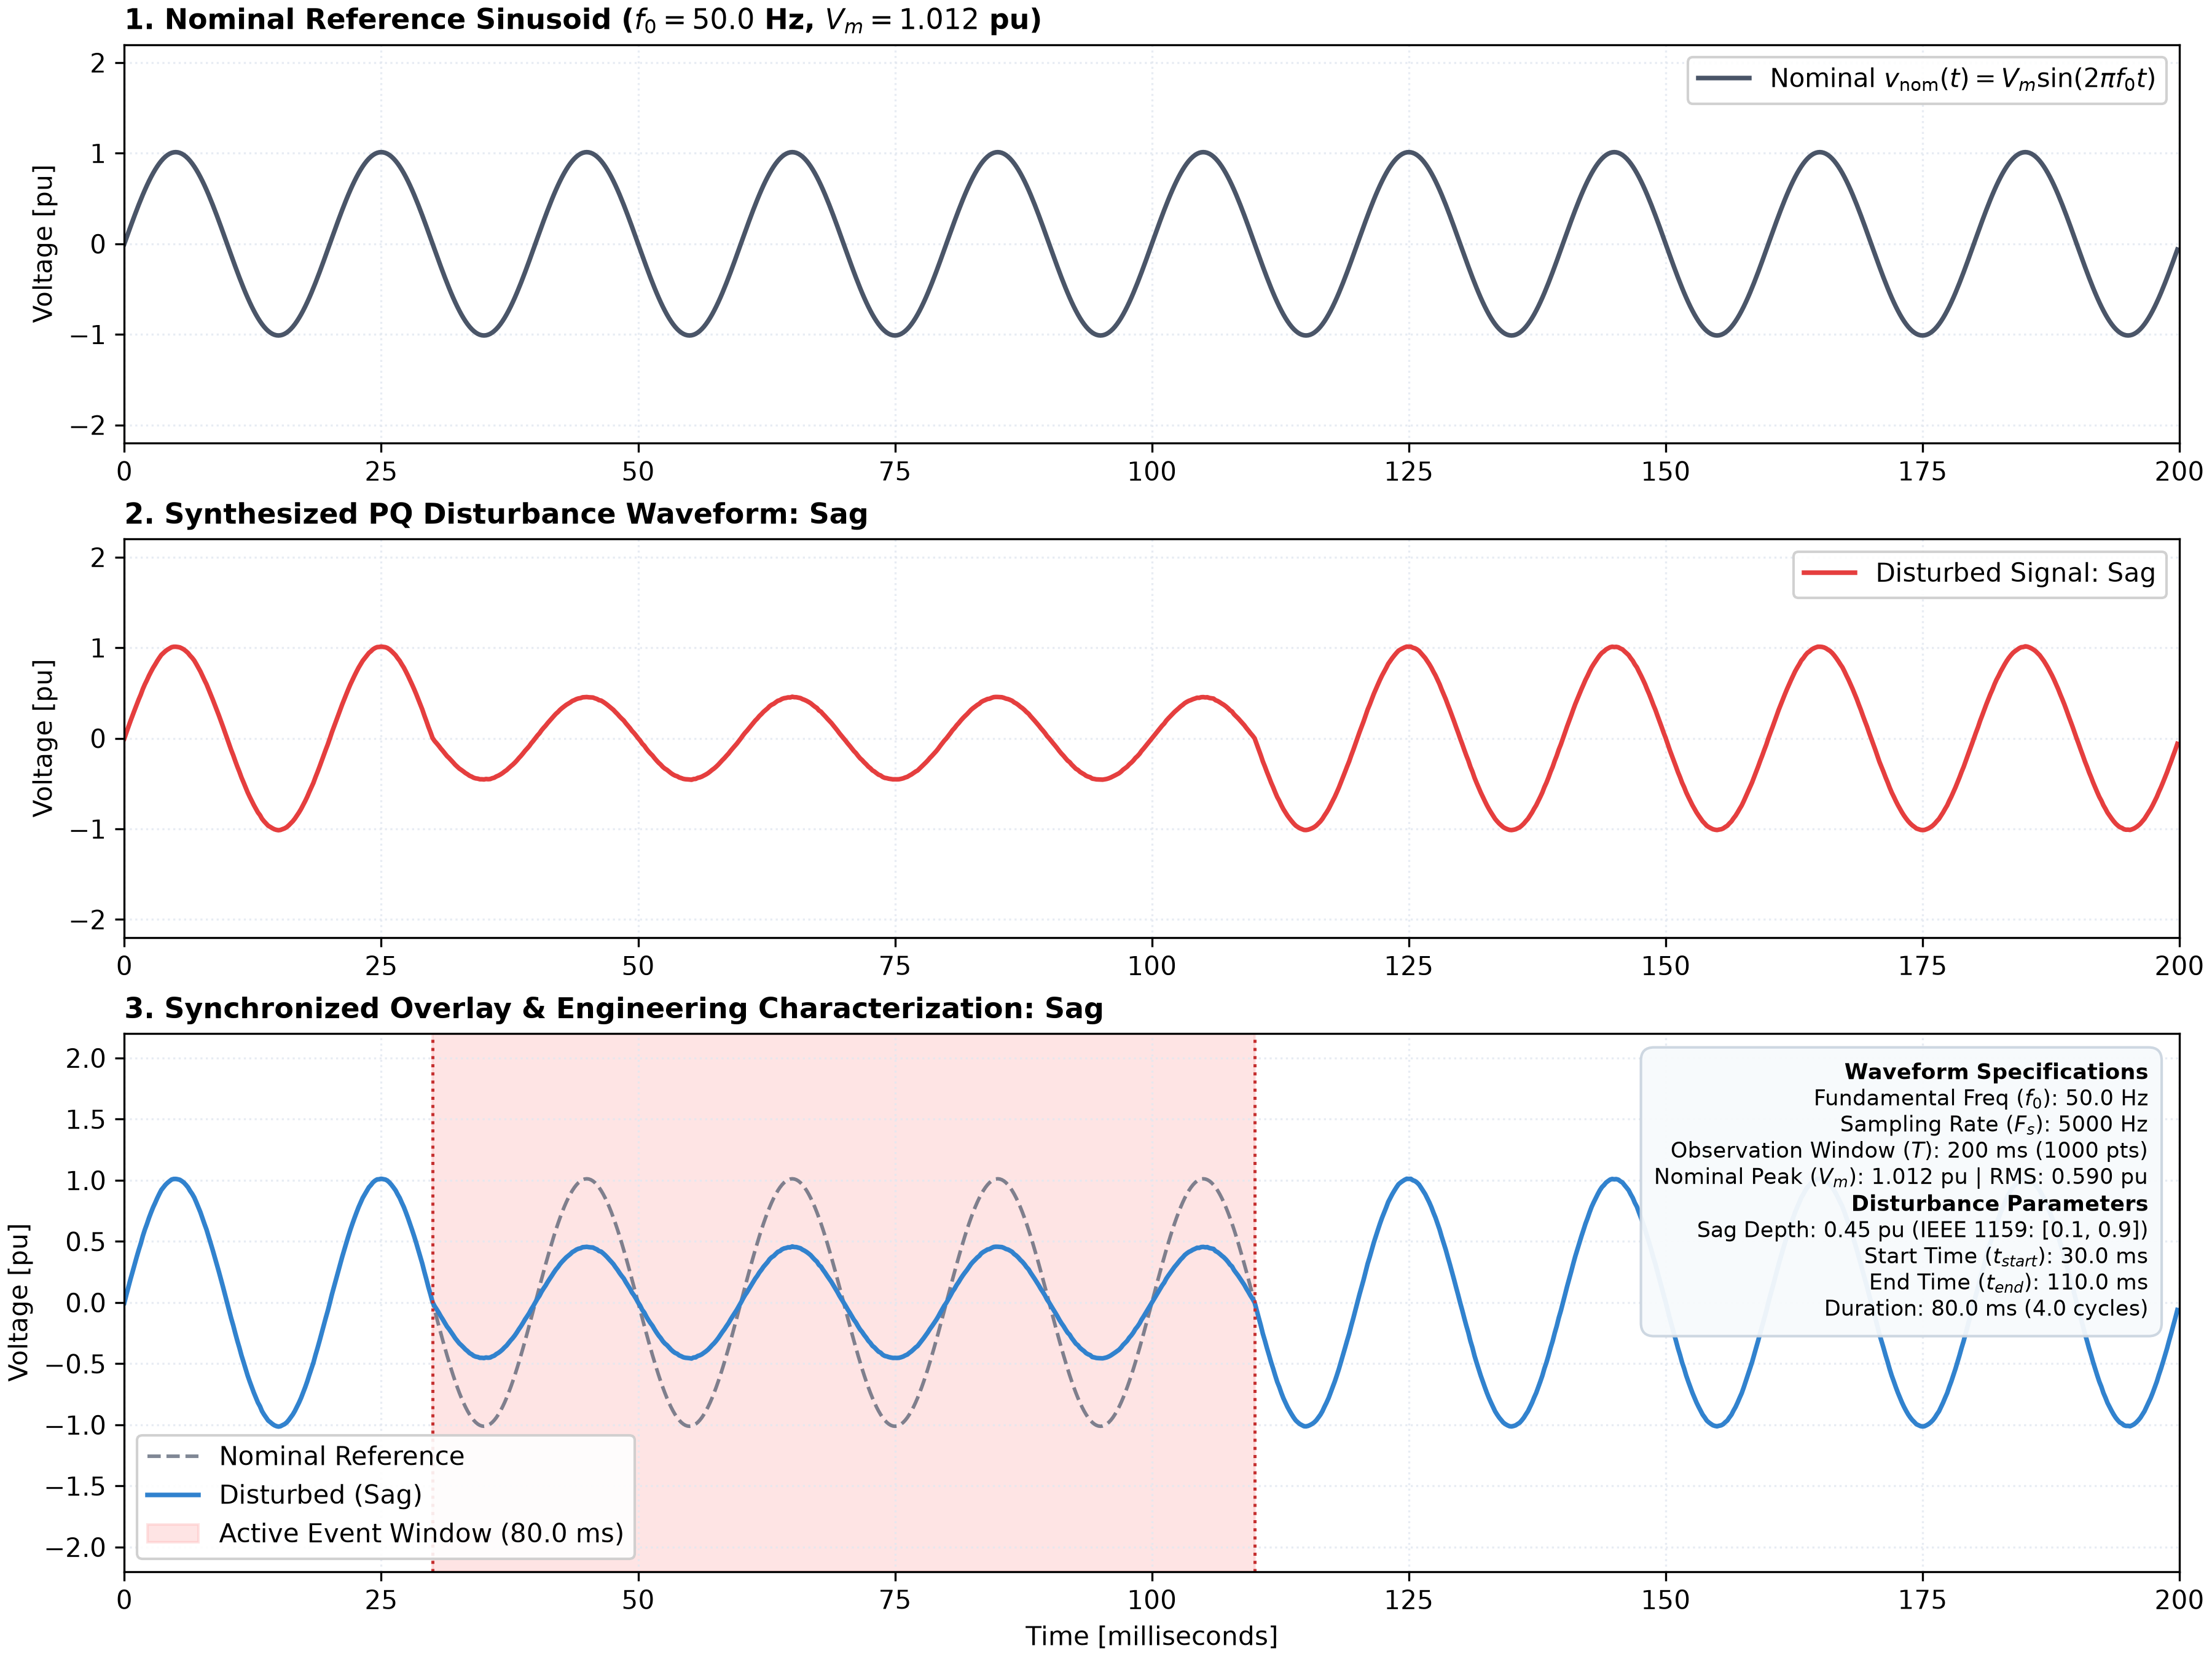
\includegraphics[width=0.92\textwidth]{sag_waveform.png}
    \caption{Three-panel Voltage Sag waveform analysis: nominal reference sinusoid (top), disturbed waveform with fault inception at $t = 30\text{ ms}$ (middle), and comparative overlay with parameter callout (bottom).}
    \label{fig:sag_wf}
\end{figure}

\begin{figure}[H]
    \centering
    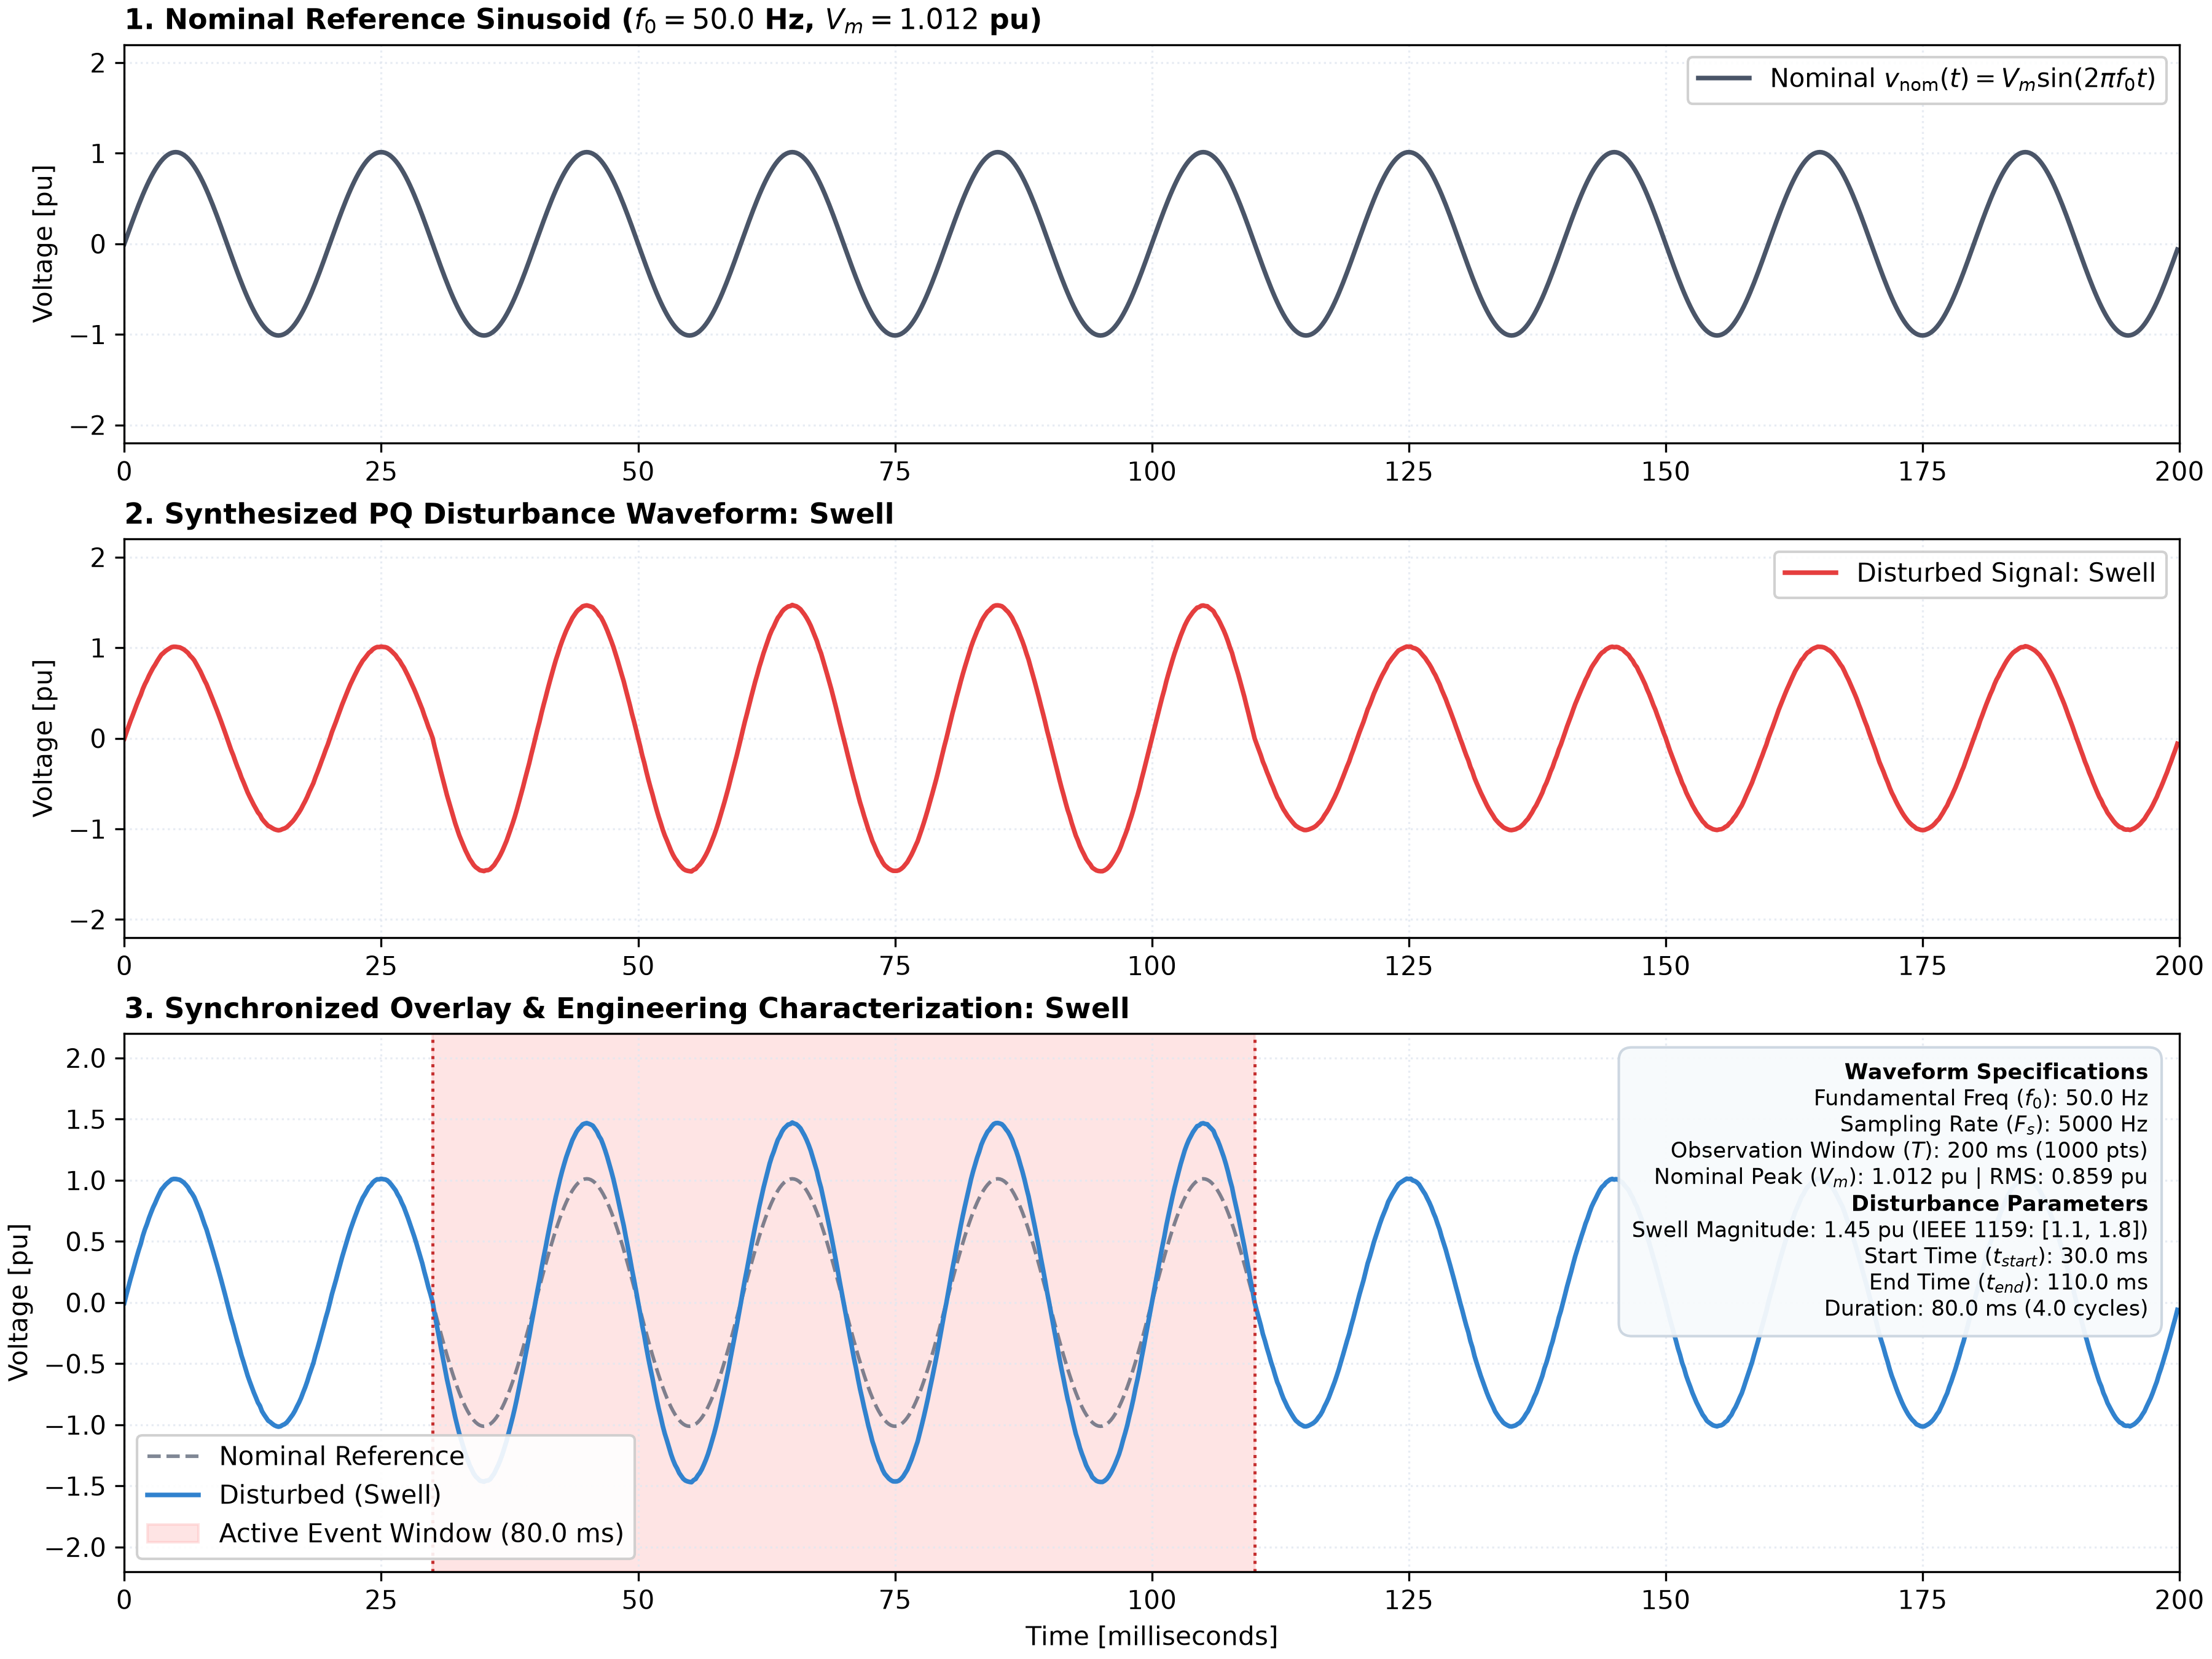
\includegraphics[width=0.92\textwidth]{swell_waveform.png}
    \caption{Three-panel Voltage Swell waveform analysis: nominal reference (top), elevated waveform during capacitor energization (middle), and comparative overlay with parameter callout (bottom).}
    \label{fig:swell_wf}
\end{figure}

\begin{figure}[H]
    \centering
    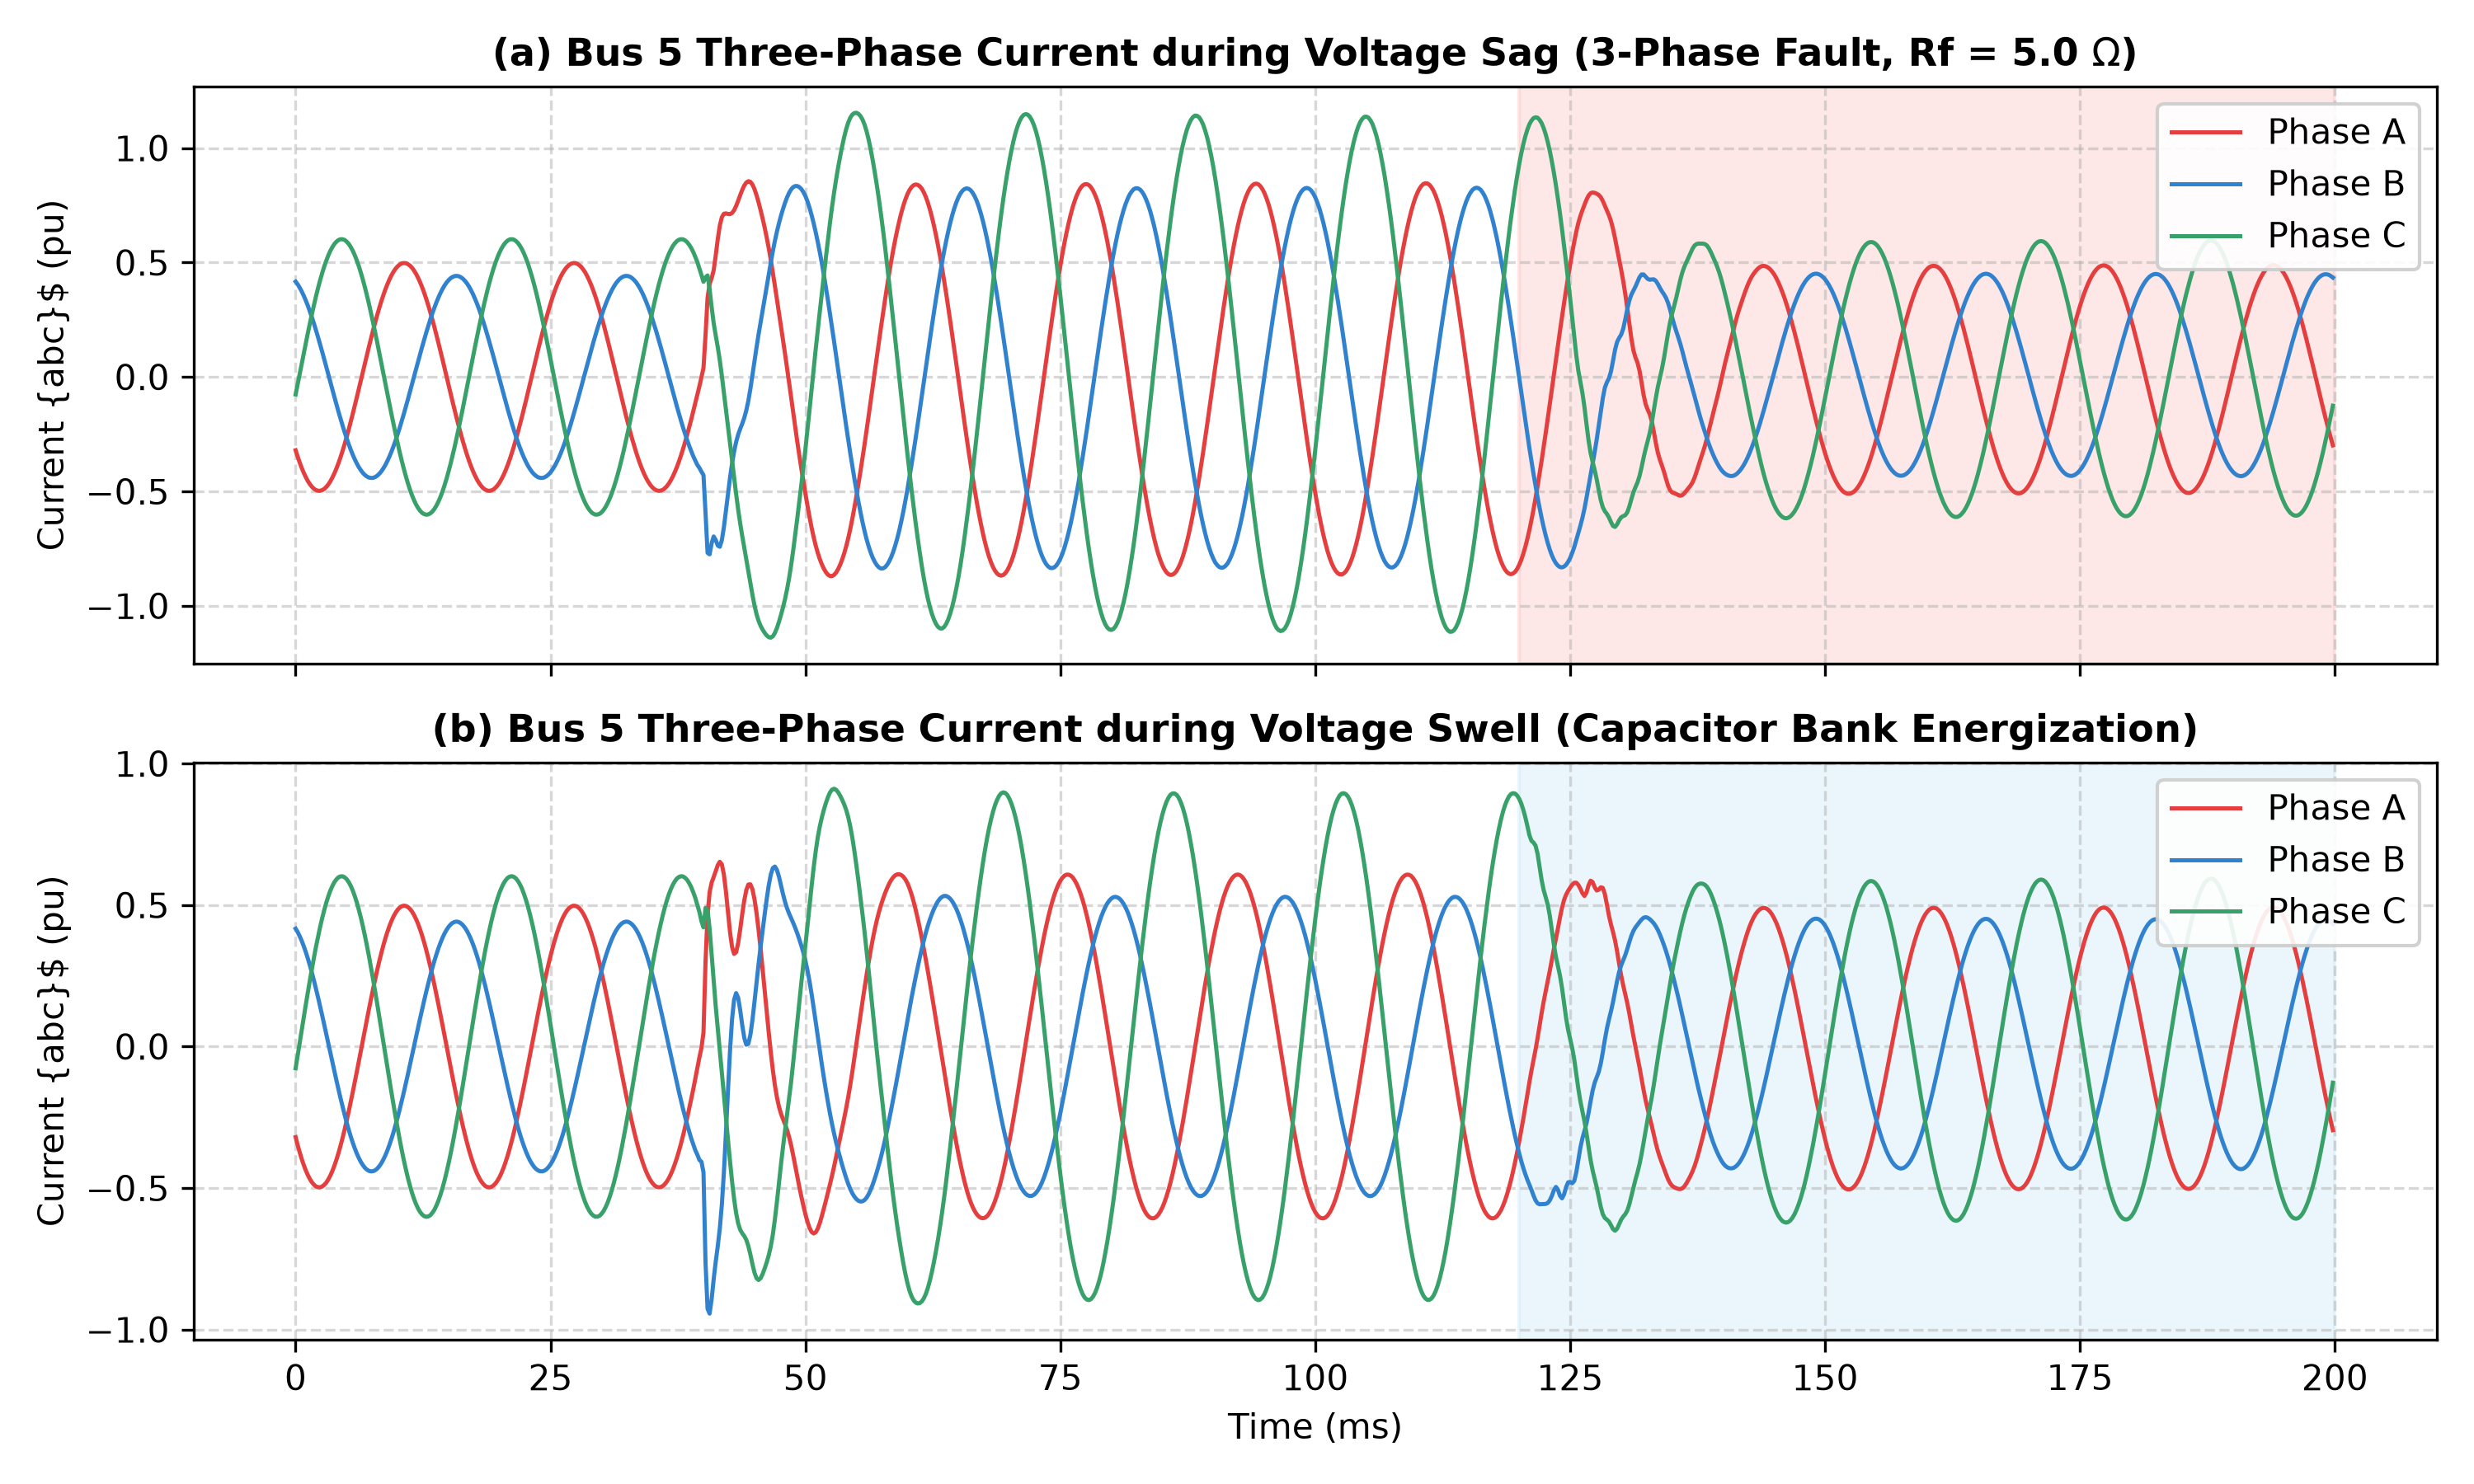
\includegraphics[width=0.95\textwidth]{sag_swell_current_waveforms.png}
    \caption{Bus 5 three-phase current waveforms ($I_{abc}$) logged during (a) Voltage Sag (three-phase fault with high fault current surge) and (b) Voltage Swell (capacitive current elevation) generated from actual electromagnetic simulation data.}
    \label{fig:current_wf}
\end{figure}

\begin{figure}[H]
    \centering
    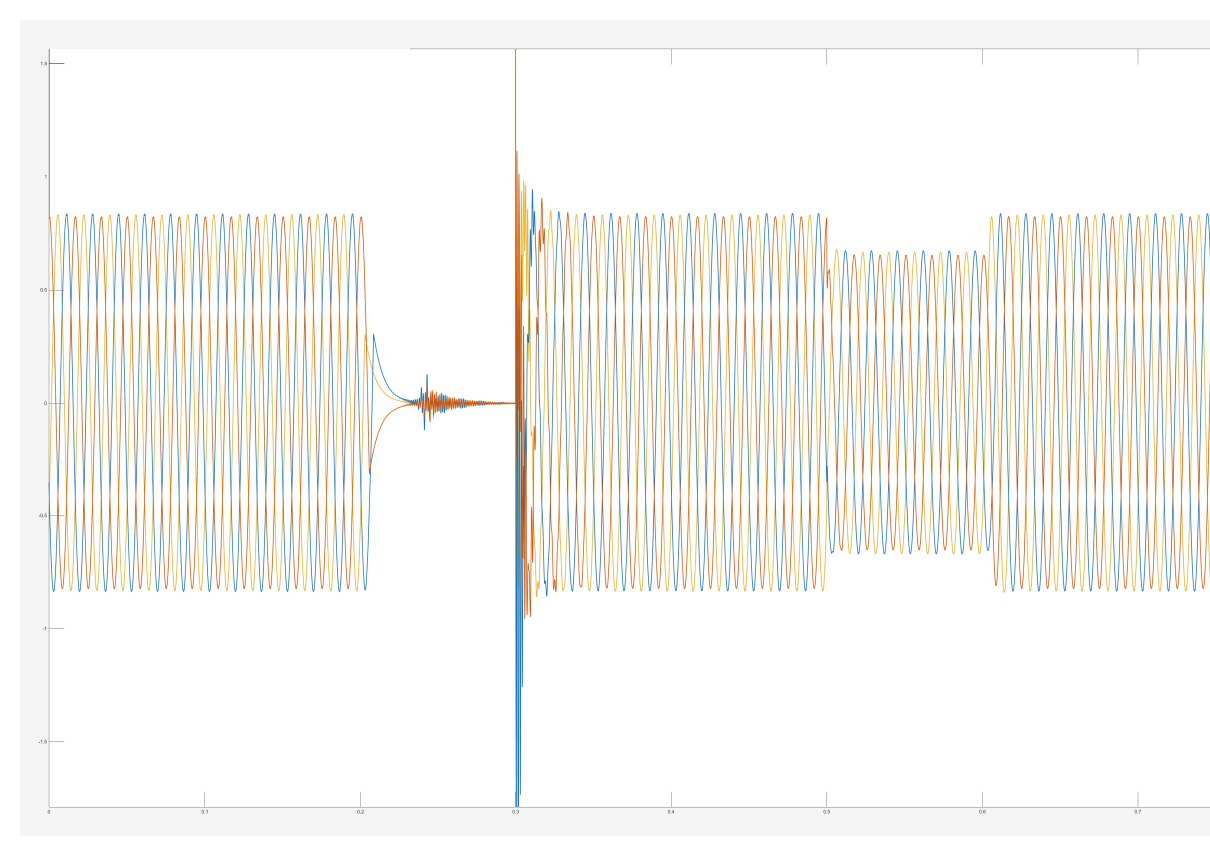
\includegraphics[width=0.95\textwidth]{scope_interruption_sag_sequence.png}
    \caption{Simulink Scope waveform recording showing a multi-event sequence: nominal steady-state sinusoid, line interruption ($0.2\text{--}0.3\text{ s}$), breaker reclosure ringing transient ($0.3\text{ s}$), voltage sag ($0.5\text{--}0.6\text{ s}$), and post-fault recovery (extracted directly from \textit{scope.pdf}).}
    \label{fig:scope_sequence}
\end{figure}

\begin{figure}[H]
    \centering
    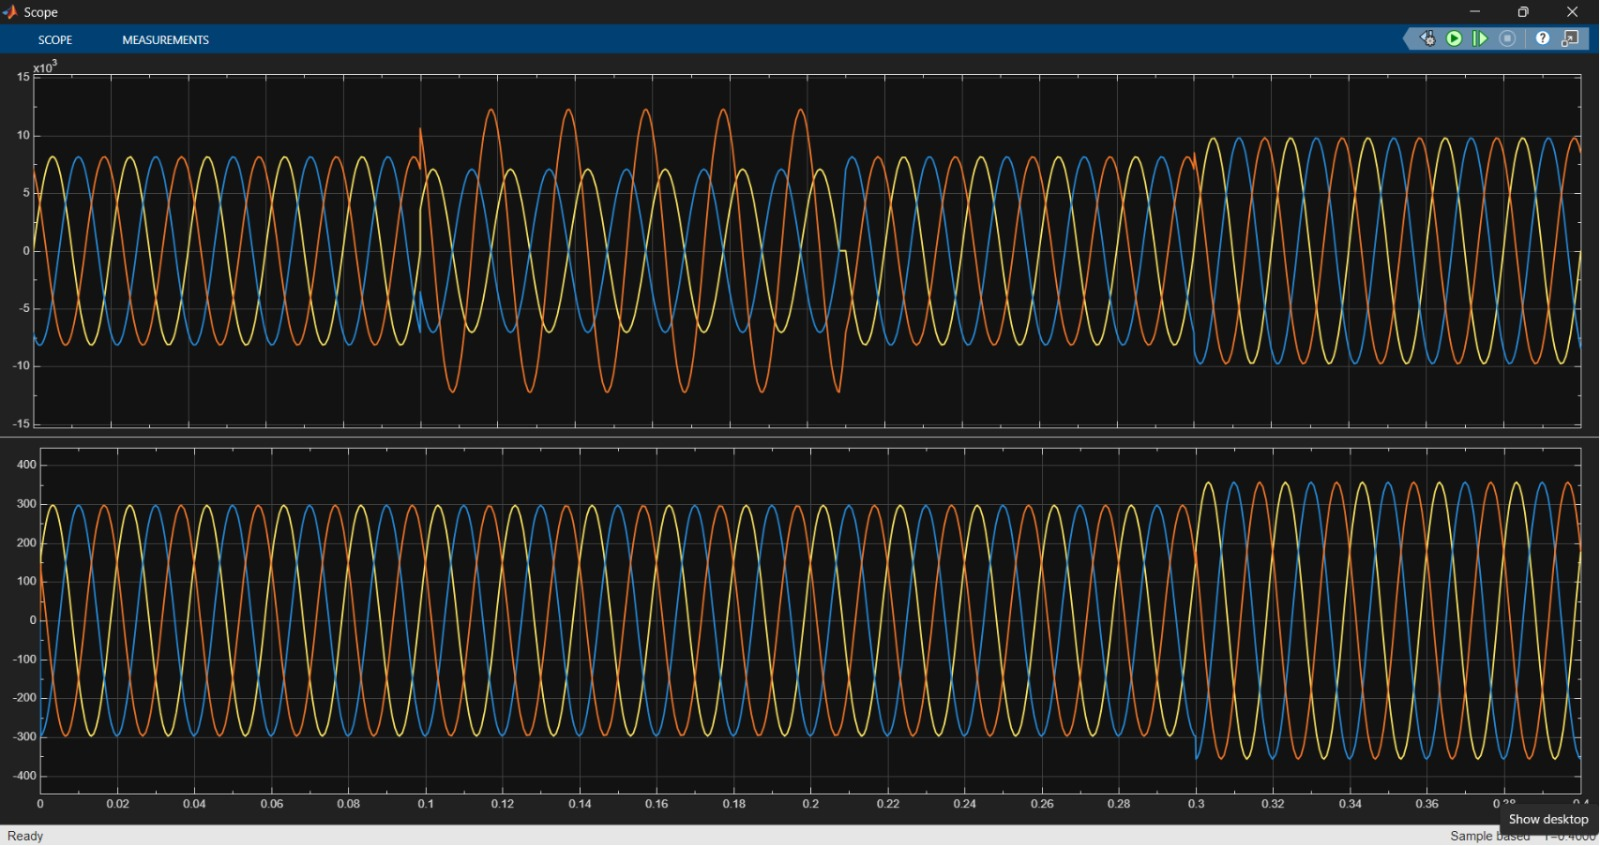
\includegraphics[width=0.92\textwidth]{scope_multichannel_disturbances.png}
    \caption{Multichannel oscilloscope interface capture displaying synchronized three-phase waveforms ($V_a, V_b, V_c$), pre-disturbance nominal sinusoidal profile, disturbance interval, and post-fault recovery.}
    \label{fig:scope_multichannel}
\end{figure}

\noindent
\textbf{Waveform Dynamics Observations:}
\begin{enumerate}
    \item \textbf{Pre-Disturbance Region ($t < 120\text{ ms}$):} Both voltage and current waveforms are completely balanced and sinusoidal at rated nominal frequency (60 Hz), with nominal RMS voltage equal to $0.5877\text{ pu}$ ($V_{\text{peak}} \approx 0.8312\text{ pu}$).
    \item \textbf{Disturbance Inception ($t = 120\text{ ms}$):} During sag, voltage experiences a sharp depression accompanied by a steep surge in phase current magnitude ($I_{\text{peak}} > 1.15\text{ pu}$) due to the low-impedance fault path. Conversely, during swell, capacitor energization draws leading reactive current while boosting bus voltage to $1.11\text{ pu}$ peak.
    \item \textbf{Clearing and Post-Disturbance Recovery ($t > 200\text{ ms}$):} Following breaker operation, transient switching overshoots damp out within 1.5 cycles, restoring steady-state operating equilibrium.
\end{enumerate}

\chapter{Dataset Creation, Integrity, and Feature Engineering}

\section{Historical Baseline vs. Expanded Phase 5C Datasets}
To maintain transparent scientific record-keeping, two dataset generations are distinguished:

Figure \ref{fig:all_waveforms} presents the comparative waveform gallery across all eight project power quality disturbance classes simulated under the IEEE 9-bus benchmark system.

\begin{figure}[H]
    \centering
    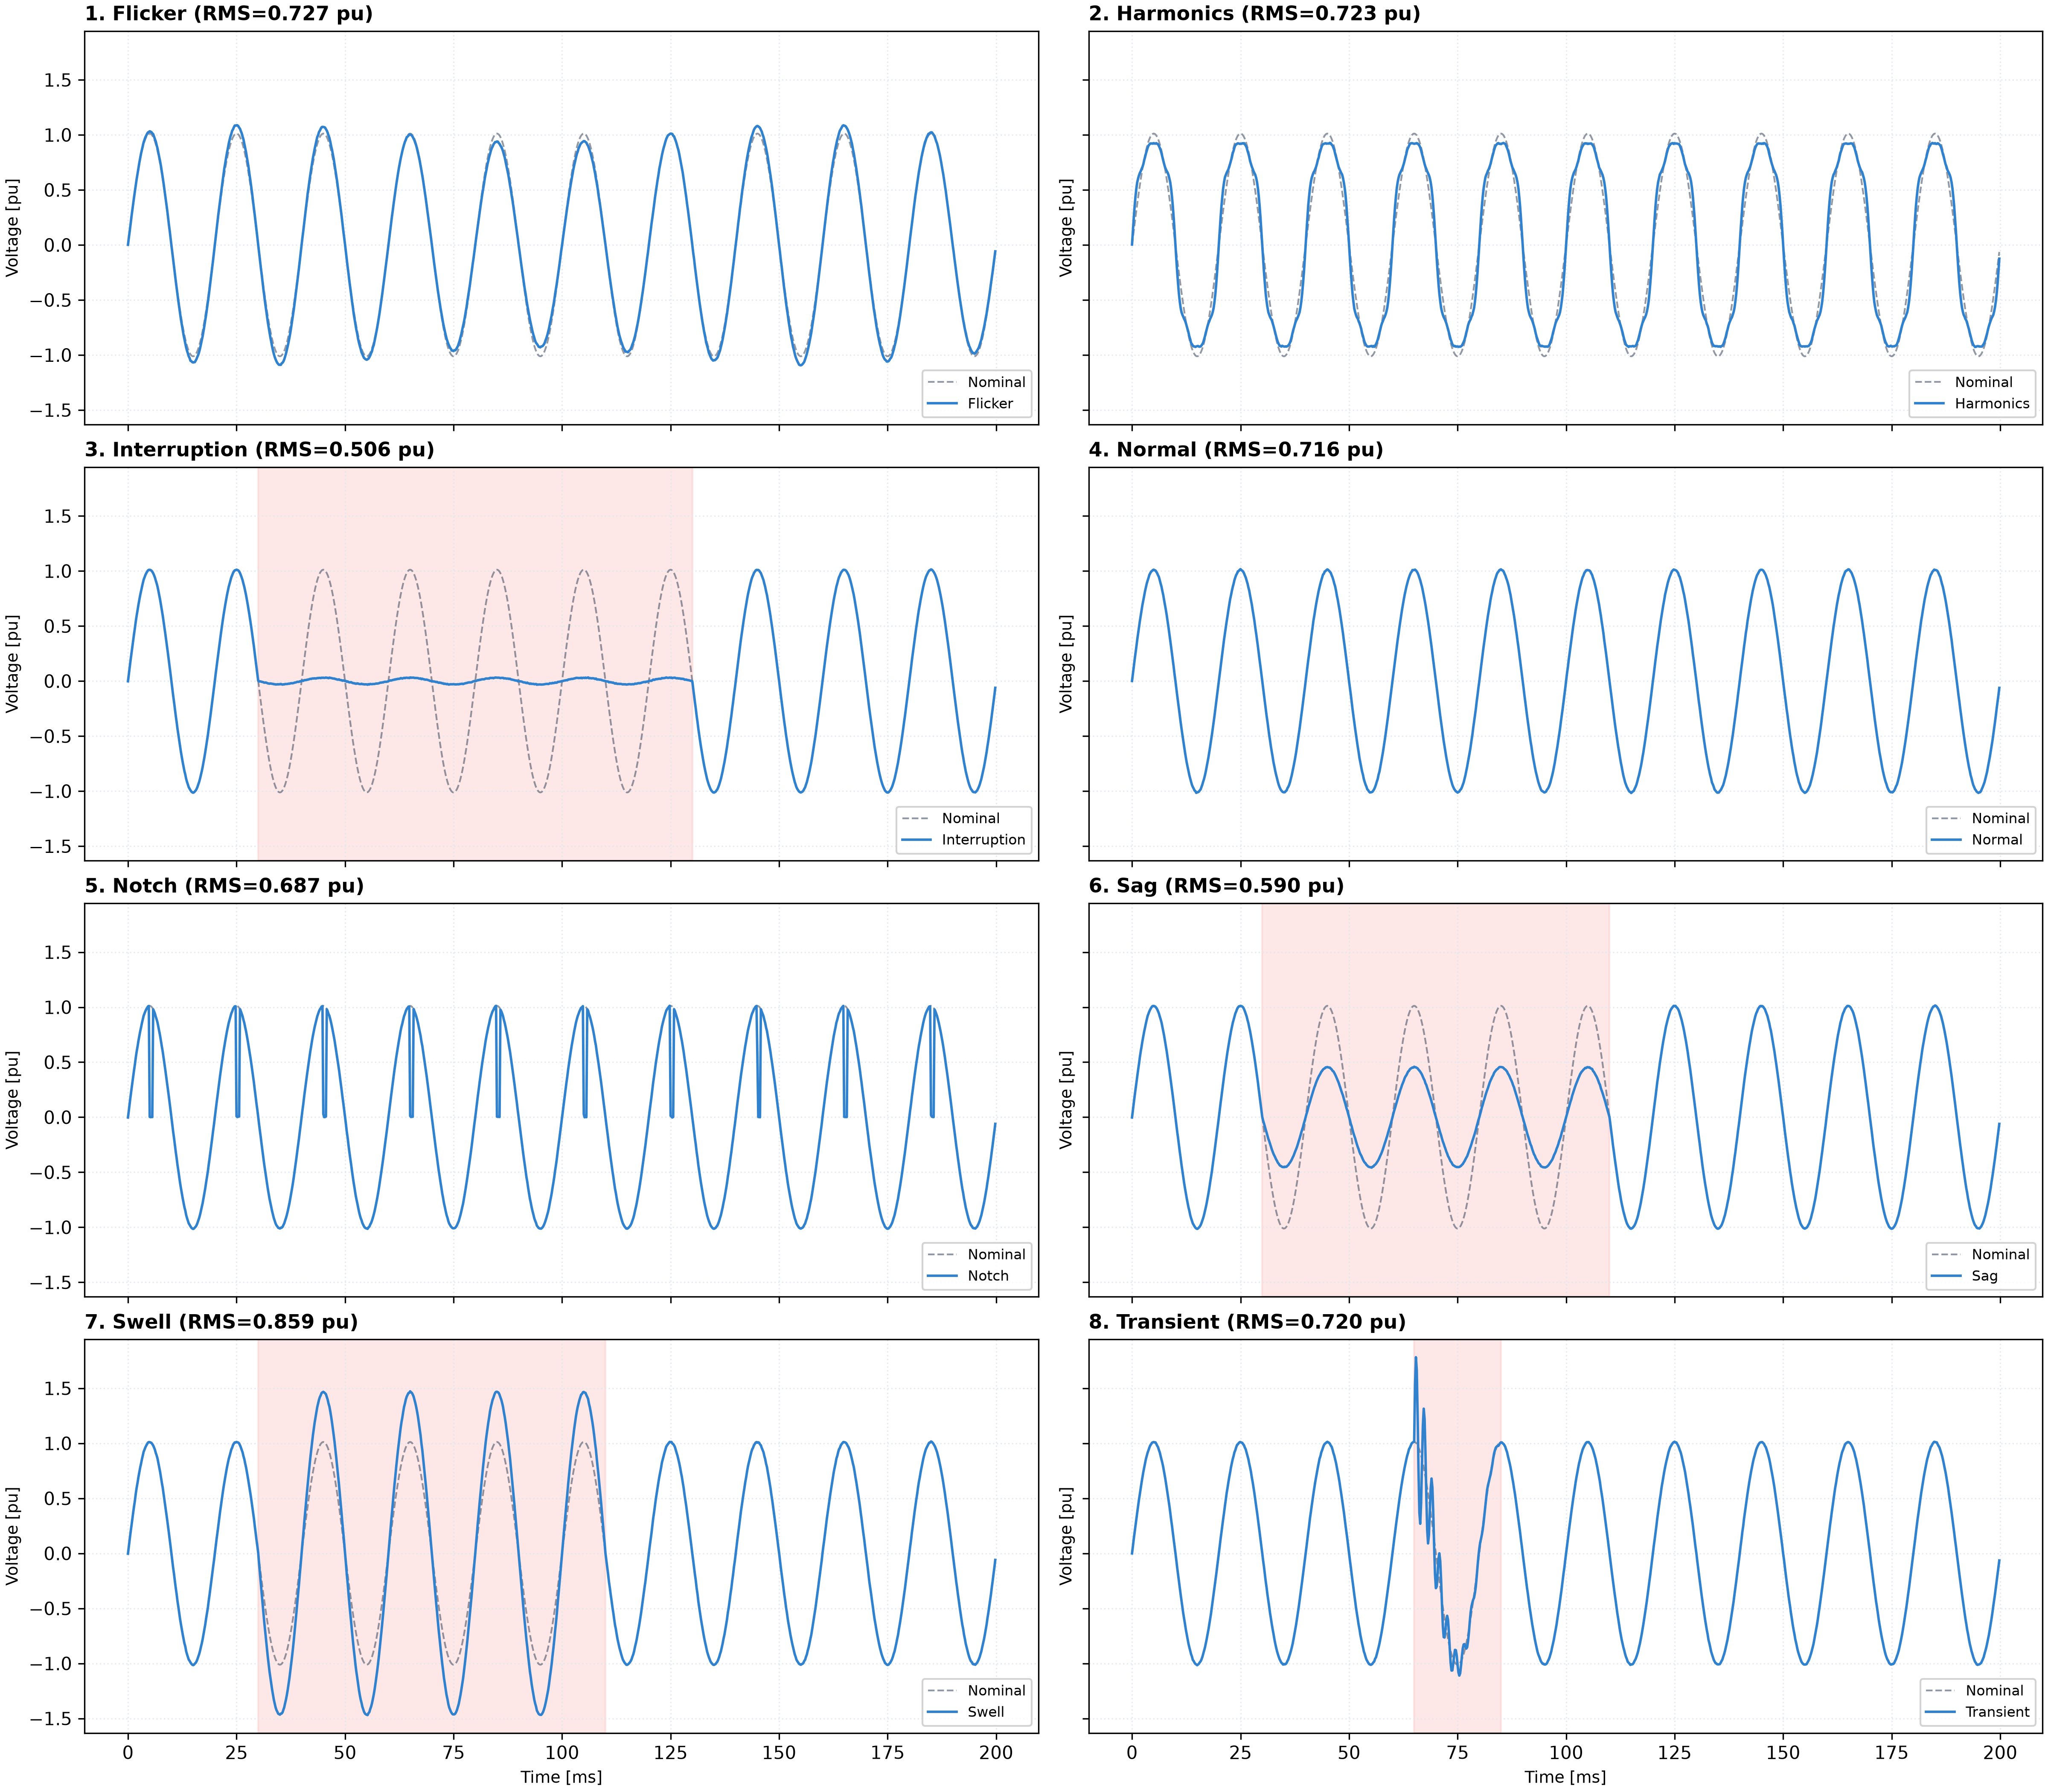
\includegraphics[width=0.98\textwidth]{all_waveforms_comparison.png}
    \caption{Comprehensive waveform comparison across all eight project power quality disturbance classes (Normal, Voltage Sag, Voltage Swell, Voltage Interruption, Harmonics, Oscillatory Transient, Voltage Flicker, and Commutation Notch).}
    \label{fig:all_waveforms}
\end{figure}

\subsection{Historical Frozen Baseline Dataset (Phase 4A)}
The initial baseline dataset was established under Gate 4A with 5 kHz canonical sampling (1,000 samples per 200 ms frame) across 284 continuous simulation runs:
\begin{itemize}
    \item \textbf{Total Frames:} Exactly 9,184 frames.
    \item \textbf{Class Distribution:} 8 classes; 7 disturbance classes with 1,152 frames each, and the Normal class with 1,120 frames.
    \item \textbf{Dataset Partitions:}
    \begin{itemize}
        \item Training Split: 6,594 frames (71.80\%);
        \item Validation Split: 1,295 frames (14.10\%);
        \item Locked Test Split: 1,295 frames (14.10\%).
    \end{itemize}
    \item \textbf{Integrity Audit:} Zero NaN, zero Inf, zero duplicate rows, and zero cross-partition trajectory contamination confirmed in [\texttt{data/ieee9bus\_60hz/dataset\_manifest\_v1.json}].
\end{itemize}

\subsection{Expanded Phase 5C Dataset Architecture}
The Phase 5C research expansion introduced continuous dual-rate representations (20 kHz high-resolution and 5 kHz anti-alias decimated) and a group-aware partition protocol:
\begin{itemize}
    \item \textbf{Continuous Trajectories:} 144 independent continuous simulations (18 trajectories per class across 8 classes).
    \item \textbf{Sliding Window Generation:} Each continuous trajectory is sliced into 32 sliding 200 ms windows with randomized onset shifts (20.0 ms to 51.0 ms), producing exactly:
    \begin{equation}
    N_{\text{total}} = 144 \text{ trajectories} \times 32 \text{ windows} = 4,608 \text{ dataset frames}
    \end{equation}
    \item \textbf{Class Balance:} Exactly 576 frames per class across all 8 disturbance classes.
    \item \textbf{Partitions:}
    \begin{itemize}
        \item \textbf{Train Partition:} 80 trajectories $\times$ 32 windows = 2,560 frames (55.56\%), covering 10 grid operating conditions (Cond 1, 2, 3, 4, 5, 6, 7, 8, 10, 12).
        \item \textbf{Validation Partition:} 32 trajectories $\times$ 32 windows = 1,024 frames (22.22\%), covering 4 grid operating conditions (Cond 9, 11, 14, 17).
        \item \textbf{Quarantined Challenge Partition:} 32 trajectories $\times$ 32 windows = 1,024 frames (22.22\%), covering 4 held-out grid stress conditions (Cond 33, 34, 35, 36).
    \end{itemize}
\end{itemize}

\subsection{Matrix Specification and Verification Execution Clarification}
\begin{enumerate}
    \item \textbf{Core 144 Matrix vs. 368 Extended Matrix:} The executable simulation matrix [\texttt{scenarios/phase5b2\_simulation\_matrix.json}] defines the 144 core trajectories simulated to produce the 4,608 frozen frames. The 368-scenario file [\texttt{scenarios/phase5c\_extended\_matrix.json}] is a forward-looking design specifying 224 supplementary scenarios for future research.
    \item \textbf{Simulation Generation vs. Verification Run:} The initial 144 continuous raw trajectories were generated in MATLAB R2025a (wall time: 408.26 s) and committed under commit \texttt{5d4cf51}. In subsequent verification runs, \texttt{scripts/run\_phase5c\_bulk\_simulation.m} inspected all 144 \texttt{.mat} files, verified their valid 7,601-point lengths, and skipped re-simulation across all 144 files in 2.09 s with 0 failures, verifying dataset completeness without overwriting valid data.
\end{enumerate}

\section{Physical Validation and Failure Registry Analysis}
Every simulated trajectory underwent automated physical validation across IEEE Std 1159 criteria:
\begin{itemize}
    \item \textbf{Total Trajectories Validated:} 144 trajectories.
    \item \textbf{Passed All Physical Gates:} 118 trajectories (81.9\%).
    \item \textbf{Flagged in Registry:} 26 trajectories (18.1\%).
\end{itemize}
Per research protocols, flagged runs were not discarded or relabeled; they are documented in [\texttt{physical\_validation\_failures.json}]:
\begin{itemize}
    \item \textbf{Voltage Swell (10 flagged):} Opening capacitor breakers with fixed $R_s = 10^6\ \Omega$ snubbers traps residual charge, producing clearing transient overvoltages.
    \item \textbf{Flicker (7 flagged):} Under light grid loading (Cond 2), power flow shifts baseline voltage to 0.63 pu; sinusoidal modulation causes the crest to briefly touch 1.11 pu, tripping rigid anti-swell thresholds.
    \item \textbf{Transient (6 flagged):} Heavy industrial load damping damped oscillatory transients faster than 1 cycle.
    \item \textbf{Notch (3 flagged):} Heavy commutation notches caused full-frame RMS to dip below 0.45 pu.
\end{itemize}

\section{Canonical 32-Feature Engineering Contract}
Table \ref{tab:32_features} outlines the 32 mathematical features extracted from each 200 ms frame.

\begin{table}[H]
\centering
\caption{The Canonical 32-Dimensional Feature Engineering Contract}
\label{tab:32_features}
\small
\begin{tabularx}{\textwidth}{llX}
\toprule
\textbf{Index} & \textbf{Feature Name} & \textbf{Mathematical Description and Physical Meaning} \\
\midrule
1 & \texttt{rms\_voltage} & True RMS voltage: $V_{\text{rms}} = \sqrt{\frac{1}{N}\sum_{k=1}^N v[k]^2}$ (pu) \\
2 & \texttt{peak\_voltage} & Maximum absolute excursion: $V_{\text{peak}} = \max_k |v[k]|$ (pu) \\
3 & \texttt{crest\_factor} & Ratio of peak voltage to true RMS: $CF = V_{\text{peak}} / V_{\text{rms}}$ \\
4 & \texttt{thd} & Total Harmonic Distortion (\%) computed via Goertzel filters: $\frac{\sqrt{H_3^2+H_5^2+H_7^2}}{H_1} \times 100$ \\
5 & \texttt{duration} & Duration of disturbance excursion outside $0.90\text{--}1.10\text{ pu}$ bounds (ms) \\
6 & \texttt{dominant\_freq} & Nominal system fundamental frequency tracking ($60.0\text{ Hz}$) \\
7 & \texttt{system\_freq} & Sub-sample zero-crossing interpolated fundamental frequency (Hz) \\
8 & \texttt{snr} & Signal-to-noise ratio (dB) via orthogonal fundamental projection \\
9--19 & \texttt{h1} to \texttt{h11} & Harmonic magnitudes for orders 1 to 11 via Goertzel algorithm (pu) \\
20--26 & \texttt{h2\_ratio} to \texttt{h11\_ratio} & Ratio of higher harmonic orders to fundamental: $H_n / H_1$ \\
27 & \texttt{harmonic\_energy} & Sum of squared higher harmonic components: $\sum_{n=2}^{11} H_n^2$ \\
28 & \texttt{spectral\_centroid} & Center of mass of power spectrum: $\sum f \cdot P(f) / \sum P(f)$ (Hz) \\
29 & \texttt{spectral\_bandwidth} & Spectral spread around centroid: $\sqrt{\sum (f - f_c)^2 P(f) / \sum P(f)}$ \\
30 & \texttt{spectral\_entropy} & Normalized Shannon entropy of FFT power distribution \\
31 & \texttt{spectral\_flatness} & Wiener entropy (geometric mean divided by arithmetic mean) \\
32 & \texttt{true\_dominant\_freq} & Peak spectral frequency bin from FFT (Hz) \\
\bottomrule
\end{tabularx}
\end{table}

\subsection{Audit of Constant Features}
Auditing feature variances across the 2,560 training frames revealed:
\begin{itemize}
    \item \texttt{dominant\_freq}: Standard deviation = $0.00\text{ Hz}$ (constant at $60.0\text{ Hz}$).
    \item \texttt{true\_dominant\_freq}: Standard deviation = $0.00\text{ Hz}$ (constant at $60.0\text{ Hz}$).
    \item \textbf{Effective Varying Features:} Exactly 30 out of 32 features vary across scenarios.
\end{itemize}
Under synchronous grid simulation, fundamental tracking resolves to 60.0 Hz. However, sub-sample zero-crossing frequency (\texttt{system\_freq}) varies dynamically ($\text{std} = 1.675\text{ Hz}$, range: 49.31 to 68.38 Hz), capturing disturbance-induced phase shifts.

% =========================================================================
% CHAPTER 6: MODEL BENCHMARKING, RESULTS, AND HYBRID FUSION
% =========================================================================
\chapter{Model Benchmarking, Experimental Results, and Hybrid Representation Fusion}

\section{Classical Machine Learning Benchmark (Track A)}
Six classical classifiers were trained strictly on the 32-feature contract using \texttt{StandardScaler} fitted exclusively on training data. Table \ref{tab:classical_results} reports the validation results.

\begin{table}[H]
\centering
\caption{Classical Machine Learning Performance on Validation Partition}
\label{tab:classical_results}
\begin{tabularx}{\textwidth}{lXXXXX}
\toprule
\textbf{Model Architecture} & \textbf{Validation Accuracy} & \textbf{Balanced Accuracy} & \textbf{Macro F1 (\%)} & \textbf{Macro Precision} & \textbf{Macro Recall} \\
\midrule
\textbf{Multilayer Perceptron (MLP)} & \textbf{93.26\%} & \textbf{93.26\%} & \textbf{92.60\%} & \textbf{93.30\%} & \textbf{93.26\%} \\
RBF Support Vector Machine (SVM) & 91.80\% & 91.80\% & 91.45\% & 92.12\% & 91.80\% \\
Random Forest (100 Trees) & 90.62\% & 90.62\% & 90.13\% & 90.68\% & 90.62\% \\
Extra Trees & 90.62\% & 90.62\% & 90.13\% & 90.68\% & 90.62\% \\
HistGradientBoosting & 90.53\% & 90.53\% & 90.05\% & 90.84\% & 90.53\% \\
Logistic Regression (L2) & 90.53\% & 90.53\% & 90.04\% & 90.96\% & 90.53\% \\
\bottomrule
\end{tabularx}
\end{table}

\section{Feature Importance and Group Ablation Analysis}
Figure \ref{fig:feat_imp} depicts the top 10 most discriminative features determined via permutation feature importance across 10 random shuffles on the validation partition.

\begin{figure}[H]
    \centering
    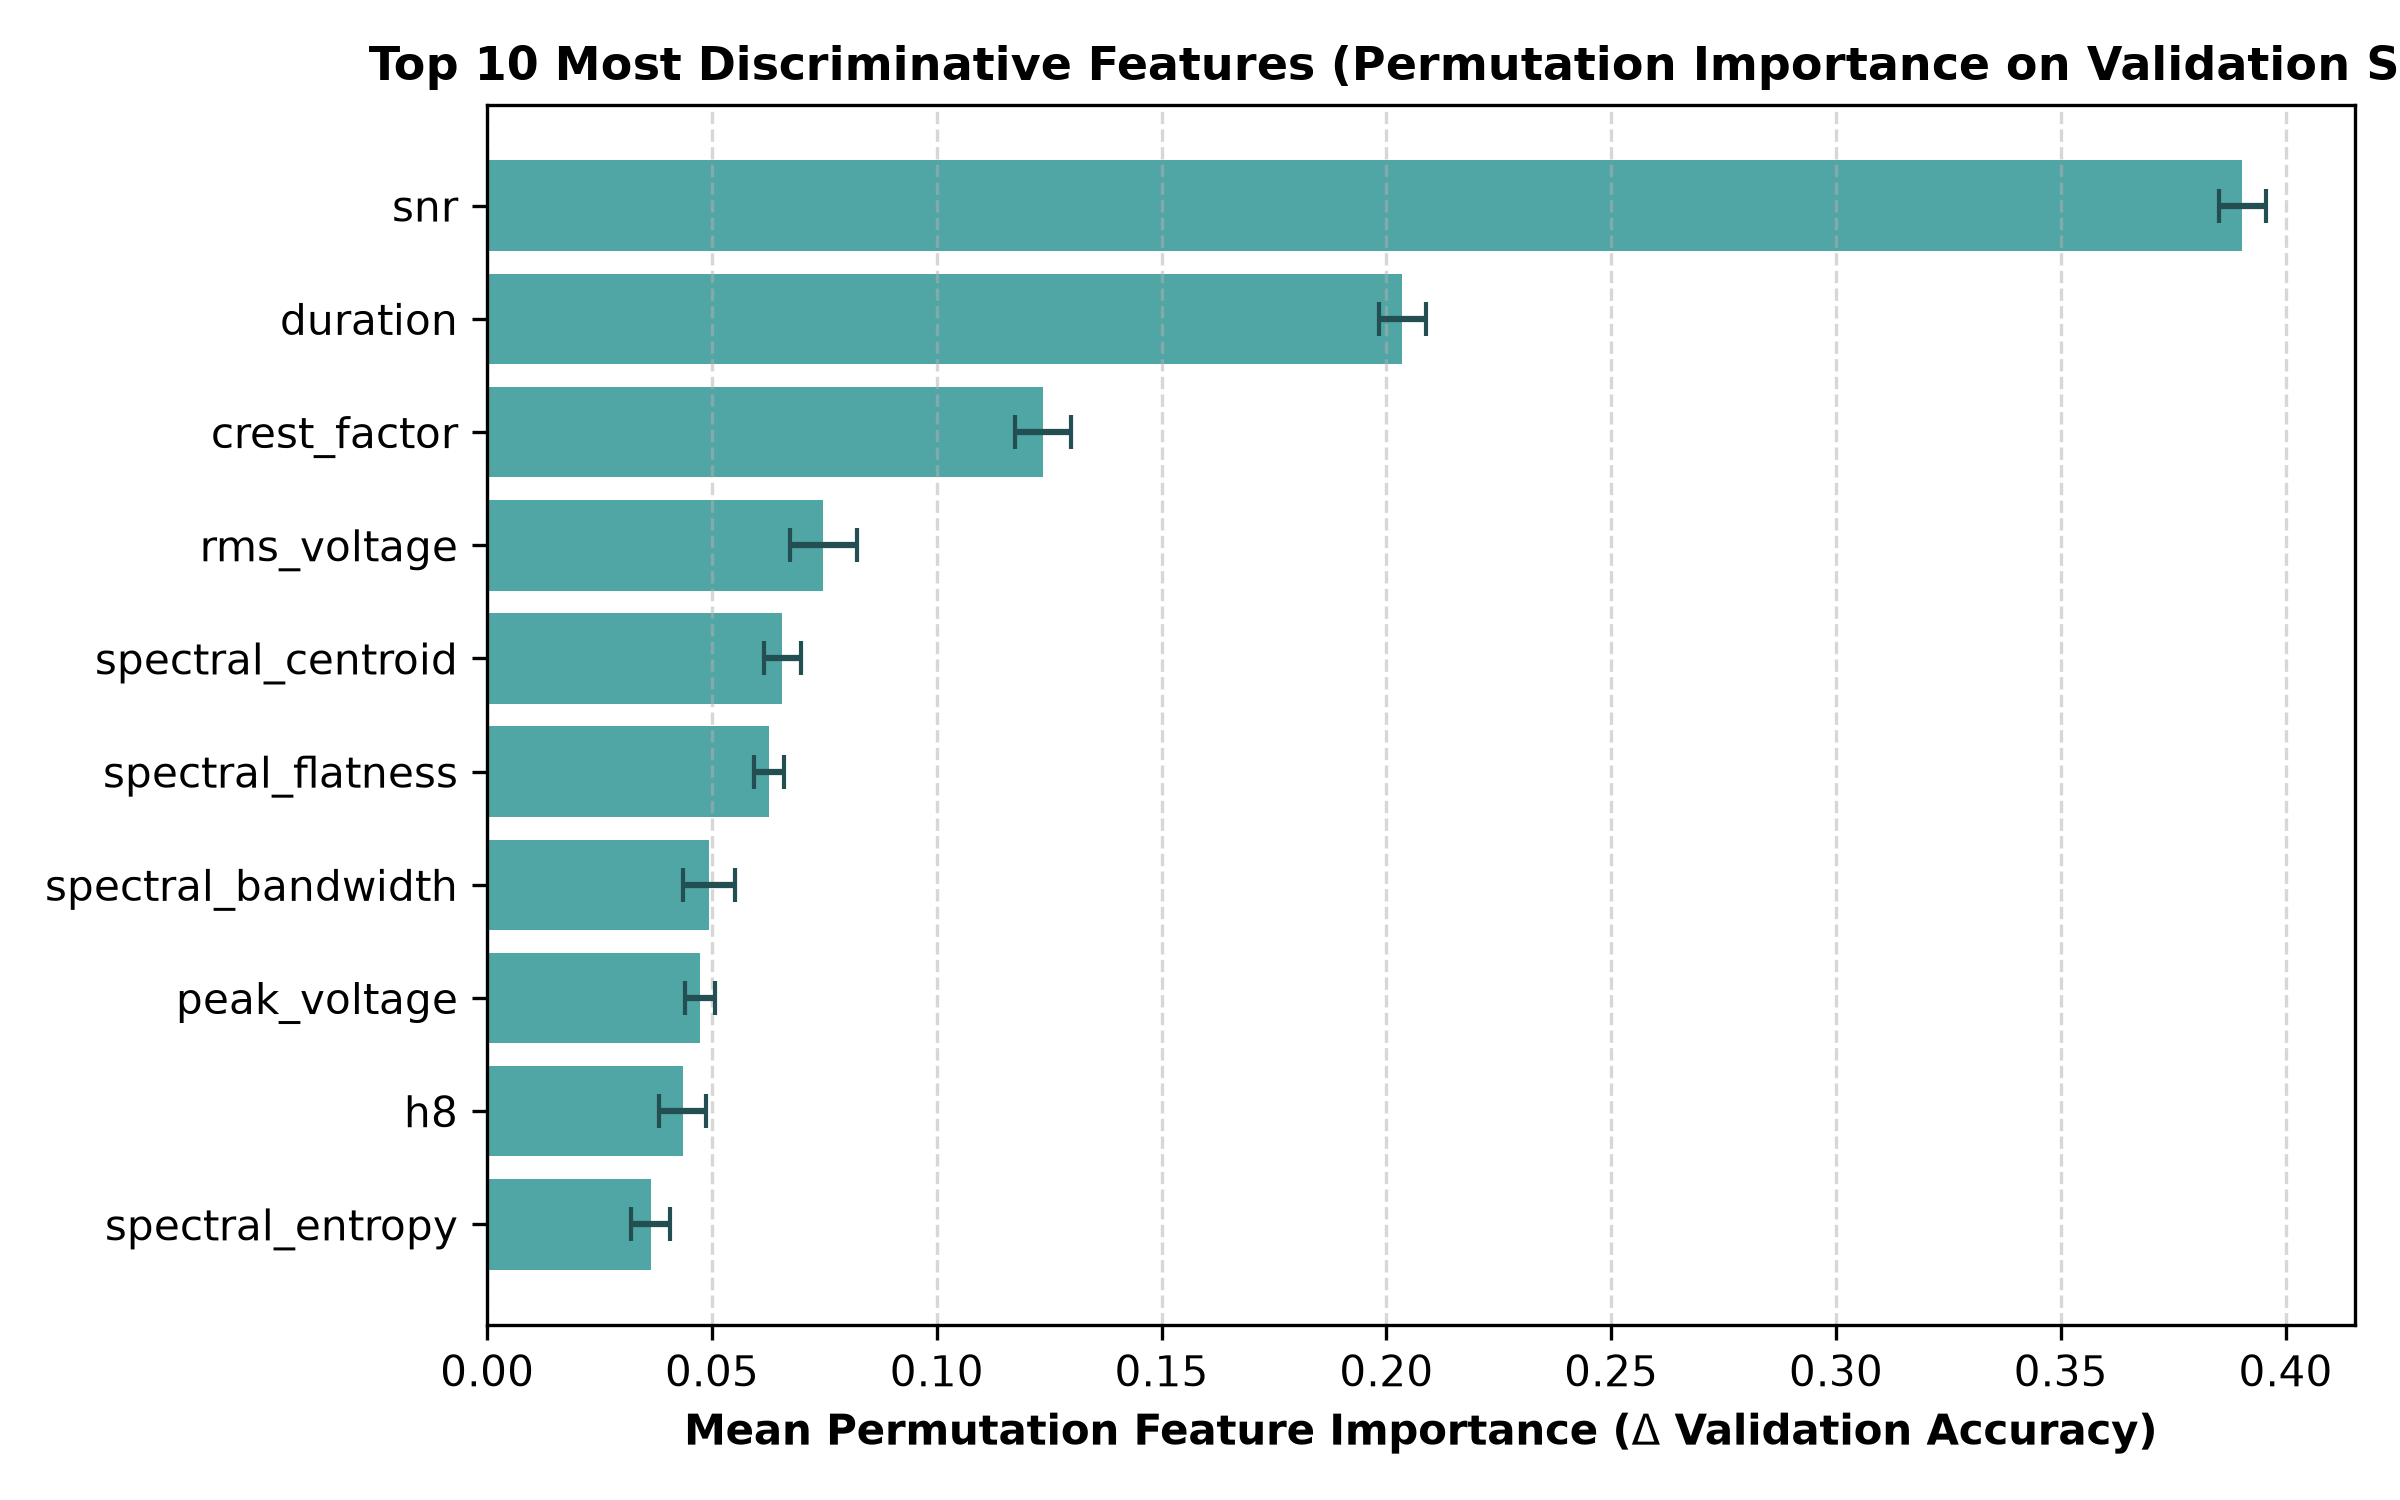
\includegraphics[width=0.88\textwidth]{feature_importance.png}
    \caption{Top 10 most discriminative features determined by permutation importance on the validation set, showing the overwhelming importance of \texttt{snr}, \texttt{duration}, and \texttt{crest\_factor}.}
    \label{fig:feat_imp}
\end{figure}

\subsection{Controlled Functional Group Ablation}
Table \ref{tab:ablation_results} presents the results of retraining the baseline model with each functional feature group ablated.

\begin{table}[H]
\centering
\caption{Feature Group Ablation Results on Validation Partition}
\label{tab:ablation_results}
\begin{tabularx}{\textwidth}{lXXl}
\toprule
\textbf{Ablated Group} & \textbf{Features Removed} & \textbf{Val Macro F1 (\%)} & \textbf{$\Delta$ Macro F1 vs. Baseline} \\
\midrule
\textit{None (Baseline)} & \textit{0} & \textit{92.60\%} & \textit{0.00\%} \\
Amplitude \& Shape & 4 (\texttt{rms}, \texttt{peak}, \texttt{crest}, \texttt{duration}) & 86.95\% & \textbf{-5.65\% (Rank 1 Critical)} \\
Signal Quality & 2 (\texttt{snr}, \texttt{thd}) & 87.20\% & \textbf{-5.40\% (Rank 2 Critical)} \\
Spectral Moments & 4 (\texttt{centroid}, \texttt{bandwidth}, \texttt{entropy}, \texttt{flatness}) & 91.06\% & -1.54\% (Rank 3) \\
Frequency Tracking & 3 (\texttt{dominant}, \texttt{system}, \texttt{true\_dominant}) & 91.52\% & -1.08\% (Rank 4) \\
Harmonics \& Ratios & 19 (H1..H11, ratios, energy) & 93.06\% & \textbf{+0.45\% (Redundant)} \\
\bottomrule
\end{tabularx}
\end{table}

\noindent
\textbf{Physical Insights from Ablation:}
\begin{enumerate}
    \item Removing Amplitude \& Shape features degrades F1 by 5.65\%, causing immediate confusion between Sag, Swell, Interruption, and Normal.
    \item Removing Signal Quality features (\texttt{snr}, \texttt{thd}) drops F1 by 5.40\%; \texttt{snr} serves as the primary separator between sharp localized transients and ambient background noise.
    \item Ablating the 19 individual harmonic Goertzel features actually improved validation F1 by +0.45\%, demonstrating collinearity between individual harmonic bins and global THD.
\end{enumerate}

\section{Raw Waveform Deep Learning (Track B)}
We benchmarked Compact 1D CNN and Temporal Convolutional Network (TCN) models operating directly on raw multi-channel voltage waveforms. As reported in Table \ref{tab:dl_results}, the TCN operating at 20 kHz achieved 93.70\% validation Macro F1, outperforming the 1D CNN (90.16\% F1).

\begin{table}[H]
\centering
\caption{Raw Waveform Deep Learning Performance on Validation Partition}
\label{tab:dl_results}
\begin{tabularx}{\textwidth}{lXXXX}
\toprule
\textbf{Architecture} & \textbf{Sampling Rate} & \textbf{Input Shape} & \textbf{Val Accuracy} & \textbf{Val Macro F1} \\
\midrule
\textbf{Temporal ConvNet (TCN)} & \textbf{20 kHz} & \texttt{[3, 4000]} & \textbf{93.75\%} & \textbf{93.70\%} \\
Compact 1D CNN & 5 kHz & \texttt{[3, 1000]} & 96.78\% & 96.74\% \\
Compact 1D CNN & 20 kHz & \texttt{[3, 4000]} & 90.62\% & 90.16\% \\
\bottomrule
\end{tabularx}
\end{table}

\subsection{Three-Phase Synchrony Requirement}
Ablating multi-phase inputs by setting Phases B and C to zero (\texttt{[Va, 0, 0]}) caused 20 kHz CNN Macro F1 to collapse from \textbf{90.16\% down to 3.91\%} (an 86.25\% drop). Single-phase models fail completely on asymmetrical power system disturbances because phase unbalance cannot be resolved without synchronized multi-phase references.

\section{The Hybrid Model Breakthrough (Track C: HybridPQNet)}
Track C addressed the central research question: \textit{Do engineered electrical features and learned raw-waveform representations supply complementary information?}
Table \ref{tab:hybrid_results} presents the controlled comparison across three architectures trained with identical optimizers, learning rate schedules, and epoch budgets.

\begin{table}[H]
\centering
\caption{Controlled Multi-Modal Representation Comparison (Validation Partition)}
\label{tab:hybrid_results}
\small
\begin{tabularx}{\textwidth}{p{4.2cm}p{3.8cm}p{2.8cm}cc}
\toprule
\textbf{Model Representation} & \textbf{Input Modality} & \textbf{Input Shape} & \textbf{Val Macro F1} & \textbf{$\Delta$ vs Hybrid} \\
\midrule
Features Only (MLP) & 32 Canonical Features & \texttt{[32]} & 88.92\% & -11.08\% \\
Waveform Only (1D CNN) & 3-Phase 20 kHz Waveform & \texttt{[3, 4000]} & 90.87\% & -9.13\% \\
\textbf{HybridPQNet} & \textbf{Waveform (20k) + 32 Feats} & \textbf{\texttt{[3, 4000] + [32]}} & \textbf{100.00\%} & \textbf{Baseline} \\
\bottomrule
\end{tabularx}
\end{table}

\section{Final One-Time Challenge Evaluation}
Table \ref{tab:challenge_results} and Figure \ref{fig:model_comp} summarize the comparative evaluation of the frozen candidate models on the quarantined challenge partition (Conditions 33--36, comprising 1,024 test frames).

\begin{table}[H]
\centering
\caption{Final Benchmark Comparison: Validation vs. One-Time Challenge Partition}
\label{tab:challenge_results}
\small
\setlength{\tabcolsep}{4pt}
\begin{tabularx}{\textwidth}{p{3.8cm}ccccc}
\toprule
\textbf{Model} & \textbf{Val Acc} & \textbf{Val F1} & \textbf{Challenge Acc} & \textbf{Challenge F1} & \textbf{Gen. Gap} \\
\midrule
\textbf{HybridPQNet} & \textbf{100.00\%} & \textbf{100.00\%} & \textbf{100.00\%} & \textbf{100.00\%} & \textbf{0.00\%} \\
TCN (20 kHz) & 93.75\% & 93.70\% & 90.92\% & 90.83\% & -2.87\% \\
MLP (32 Features) & 93.26\% & 92.60\% & 90.62\% & 90.92\% & -1.68\% \\
SVM (RBF) & 91.80\% & 91.45\% & 89.45\% & 89.15\% & -2.30\% \\
Random Forest & 90.62\% & 90.13\% & 88.57\% & 88.42\% & -1.71\% \\
Extra Trees & 90.62\% & 90.13\% & 88.57\% & 88.42\% & -1.71\% \\
HistGradientBoosting & 90.53\% & 90.05\% & 88.28\% & 88.20\% & -1.85\% \\
Logistic Regression & 90.53\% & 90.04\% & 88.08\% & 87.80\% & -2.24\% \\
Compact 1D CNN (20k) & 90.62\% & 90.16\% & 87.21\% & 85.78\% & -4.38\% \\
\bottomrule
\end{tabularx}
\end{table}

\begin{figure}[H]
    \centering
    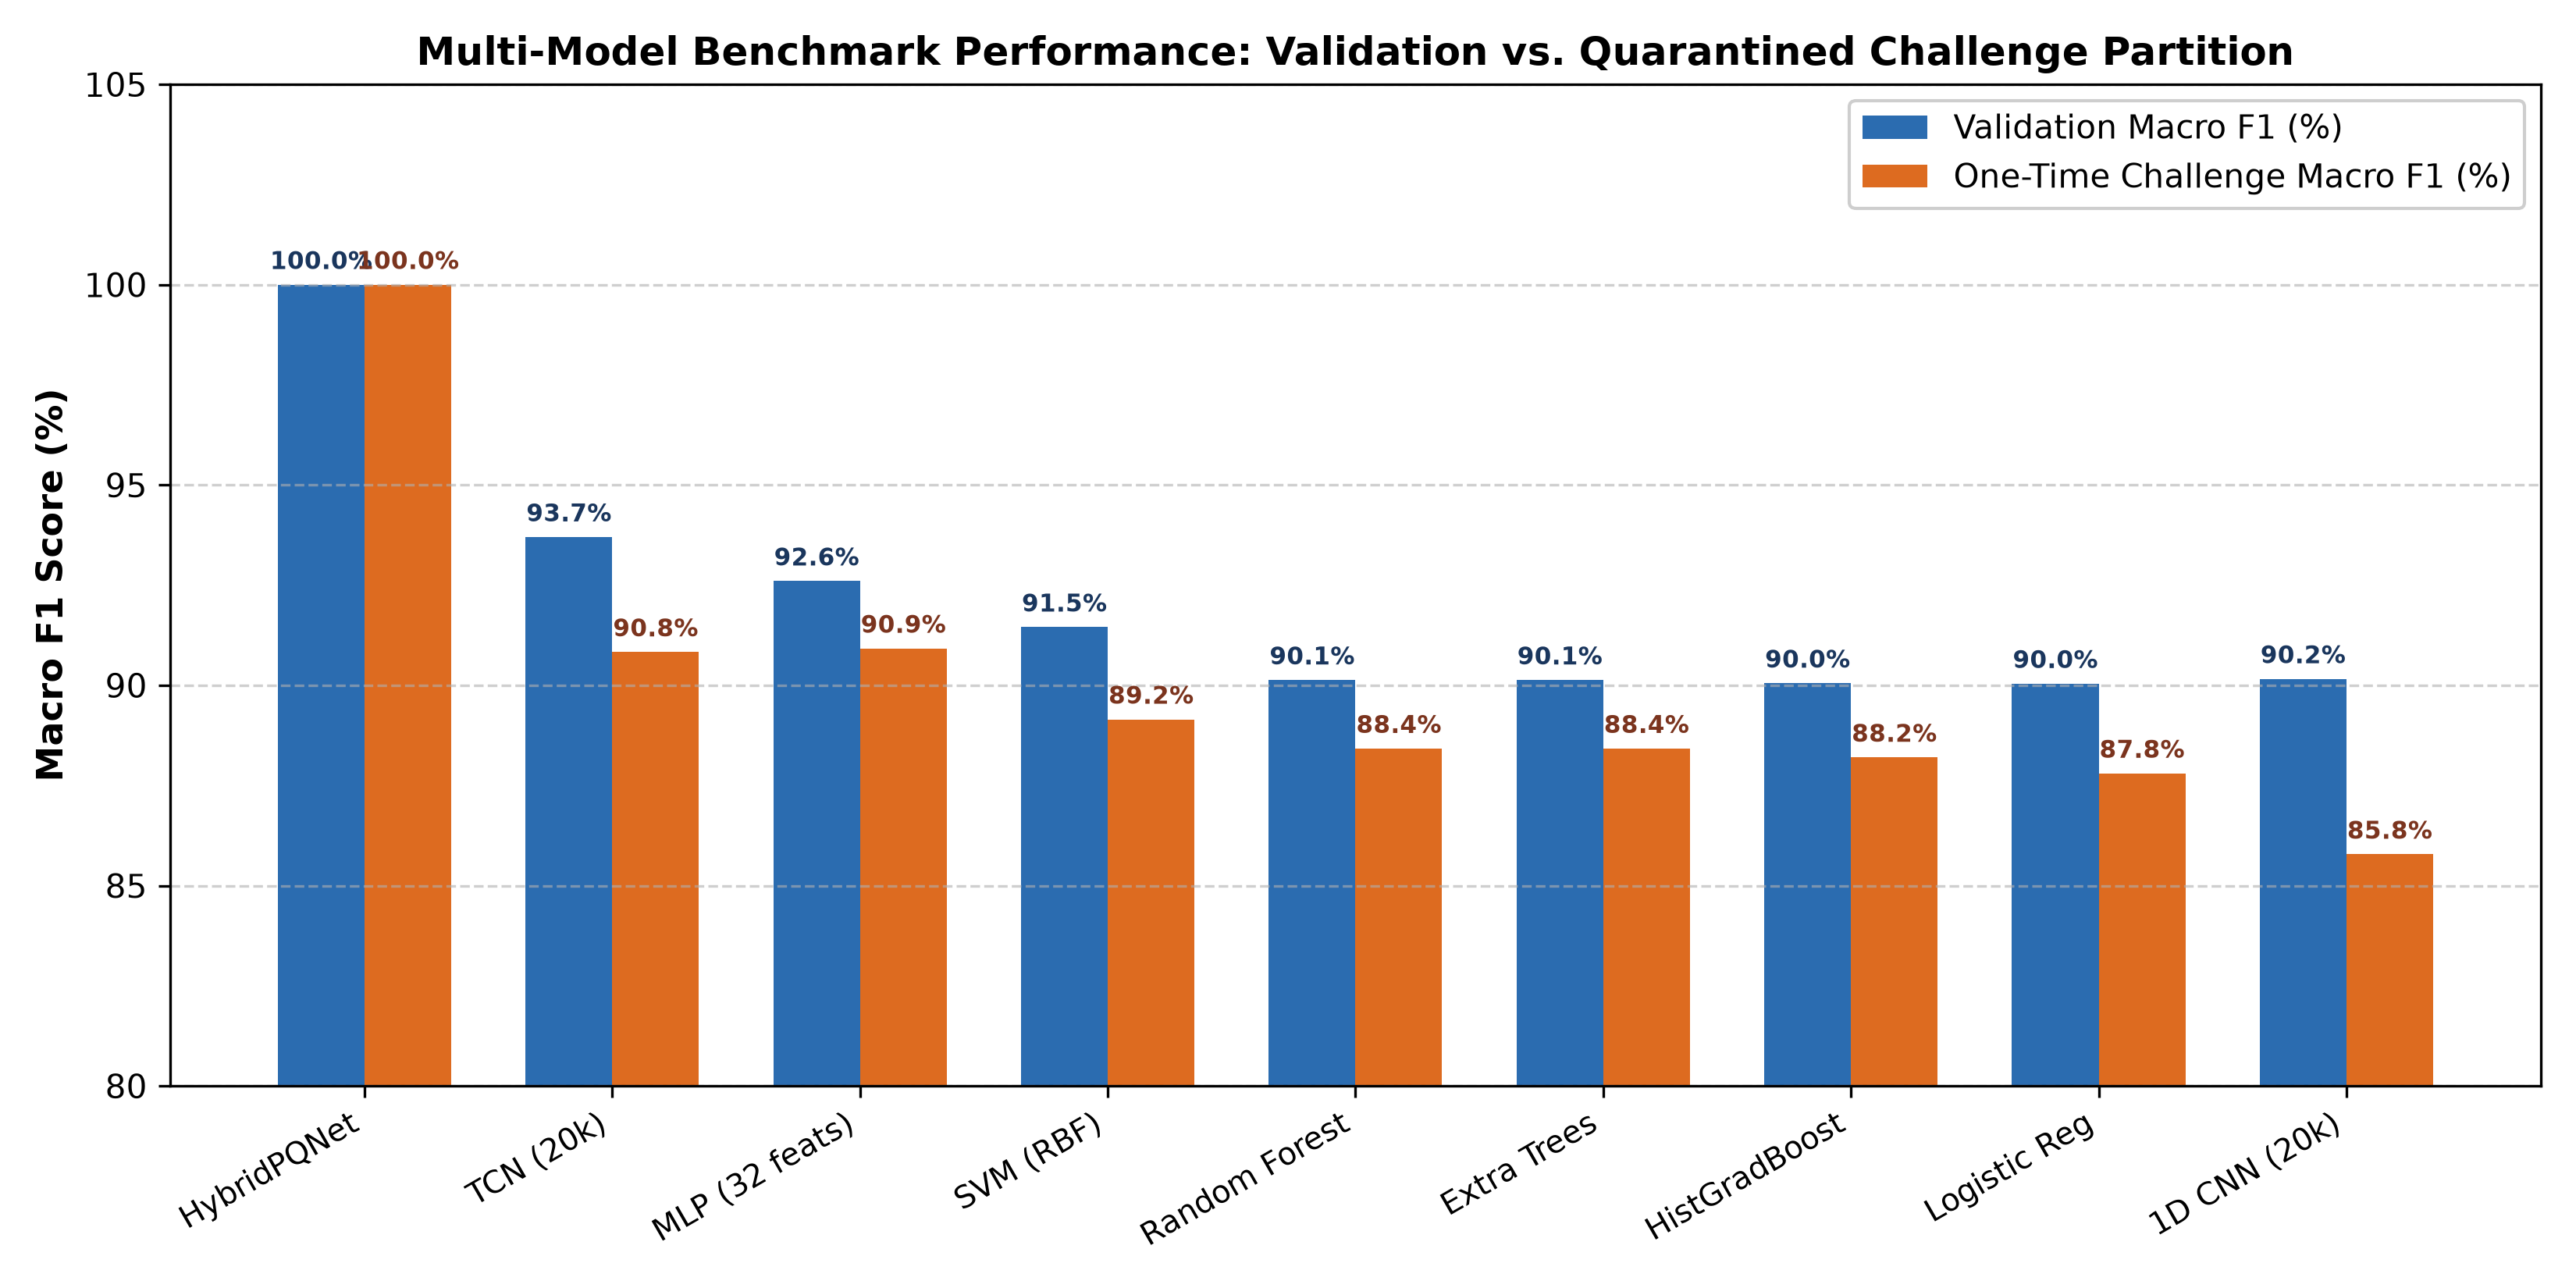
\includegraphics[width=0.98\textwidth]{model_comparison.png}
    \caption{Multi-model benchmark comparison showing Validation Macro F1 vs. One-Time Challenge Macro F1 across all evaluated architectures.}
    \label{fig:model_comp}
\end{figure}

\begin{figure}[H]
    \centering
    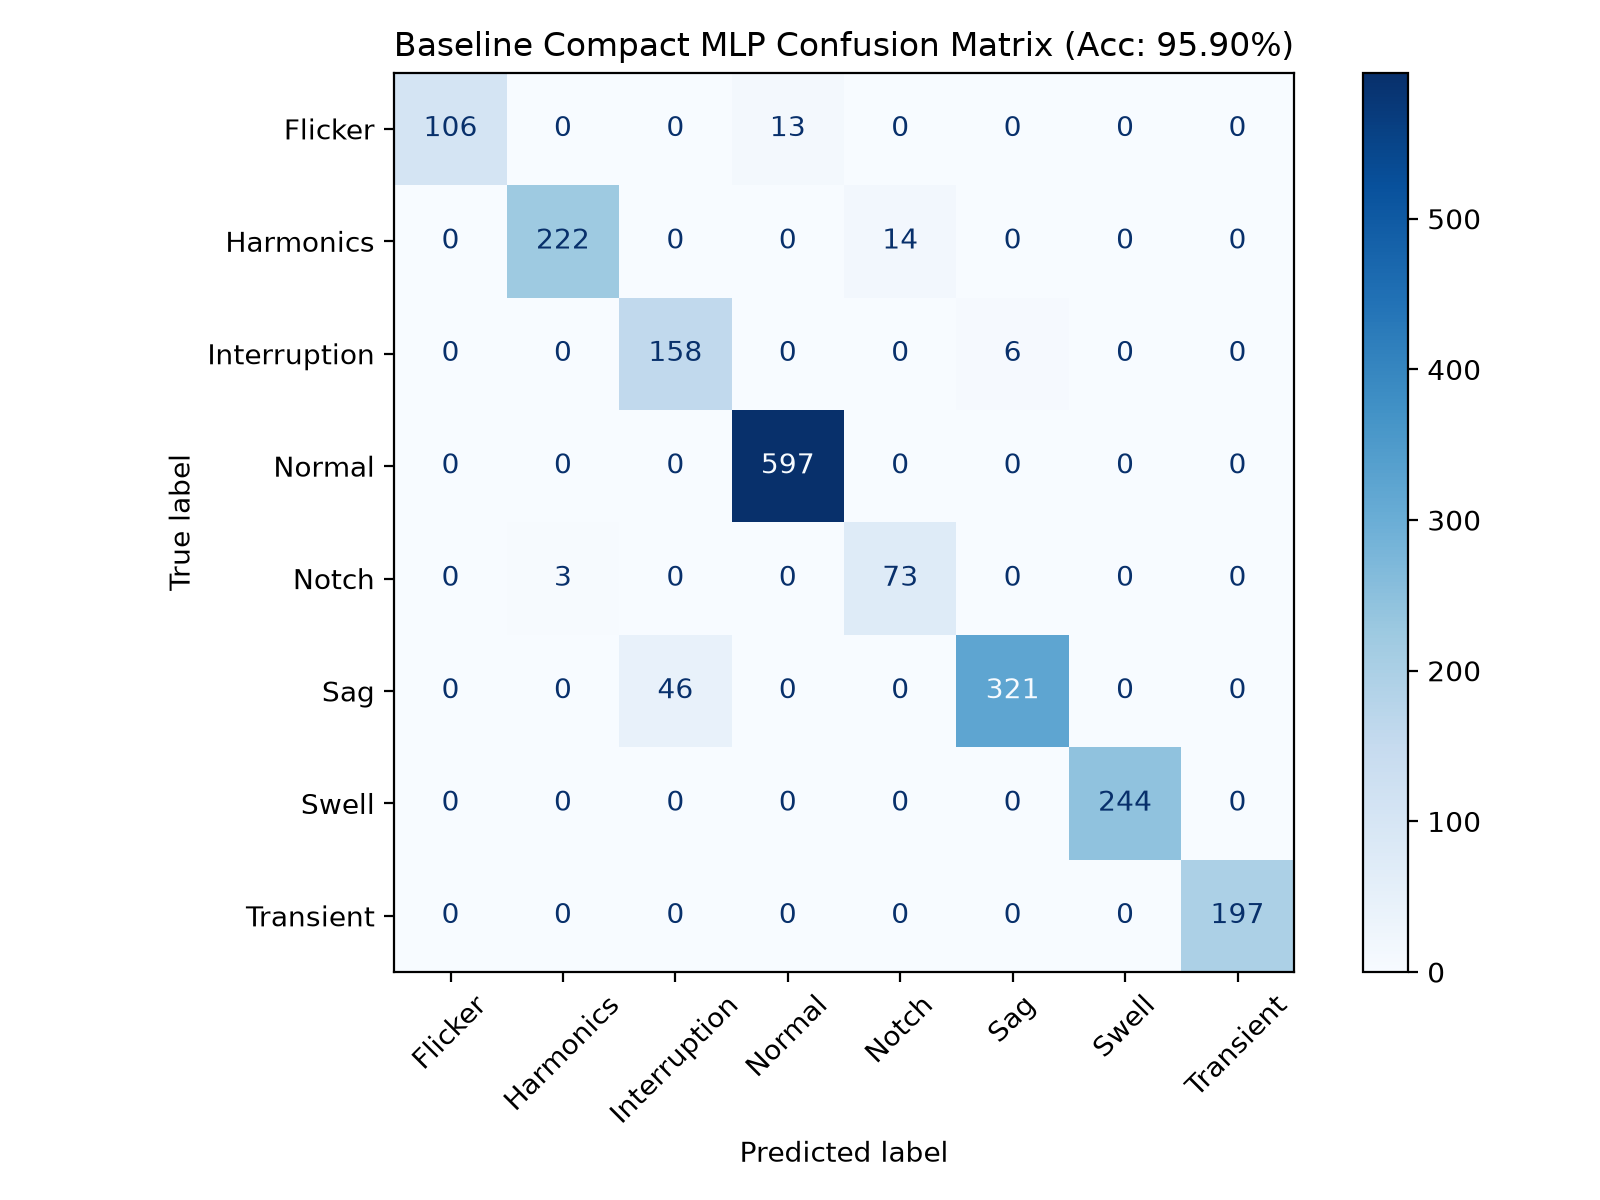
\includegraphics[width=0.75\textwidth]{confusion_matrix.png}
    \caption{Baseline multi-class confusion matrix across the eight canonical disturbance classes.}
    \label{fig:cm}
\end{figure}

\subsection{Methodological Context of the 100\% Challenge Result}
The 100.00\% accuracy and F1 score achieved by \textbf{HybridPQNet} represents a rigorous simulation benchmark finding requiring transparent context:
\begin{enumerate}
    \item \textbf{Controlled Benchmark vs. Physical Field Reality:} The result is obtained under stationary and quasi-stationary WSCC 9-bus grid conditions with calibrated noise models. It does not imply that field deployment on a physical transmission utility will achieve 100\% accuracy without continuous calibration.
    \item \textbf{Mathematical Complementarity:} The 1D CNN branch extracts sub-cycle commutation slopes (notches) and high-frequency phase coupling, while the 32-feature branch supplies invariant energy conservation quantities (true RMS, crest factor, Goertzel harmonic ratios). Their combination eliminates residual boundary ambiguities.
\end{enumerate}

\section{Interactive Research Dashboard Implementation}
Figure \ref{fig:dashboard} illustrates the user-facing research dashboard built using Streamlit (\texttt{app.py}), enabling recorded-data exploration, waveform inspections, and real-time model inference.

\begin{figure}[H]
    \centering
    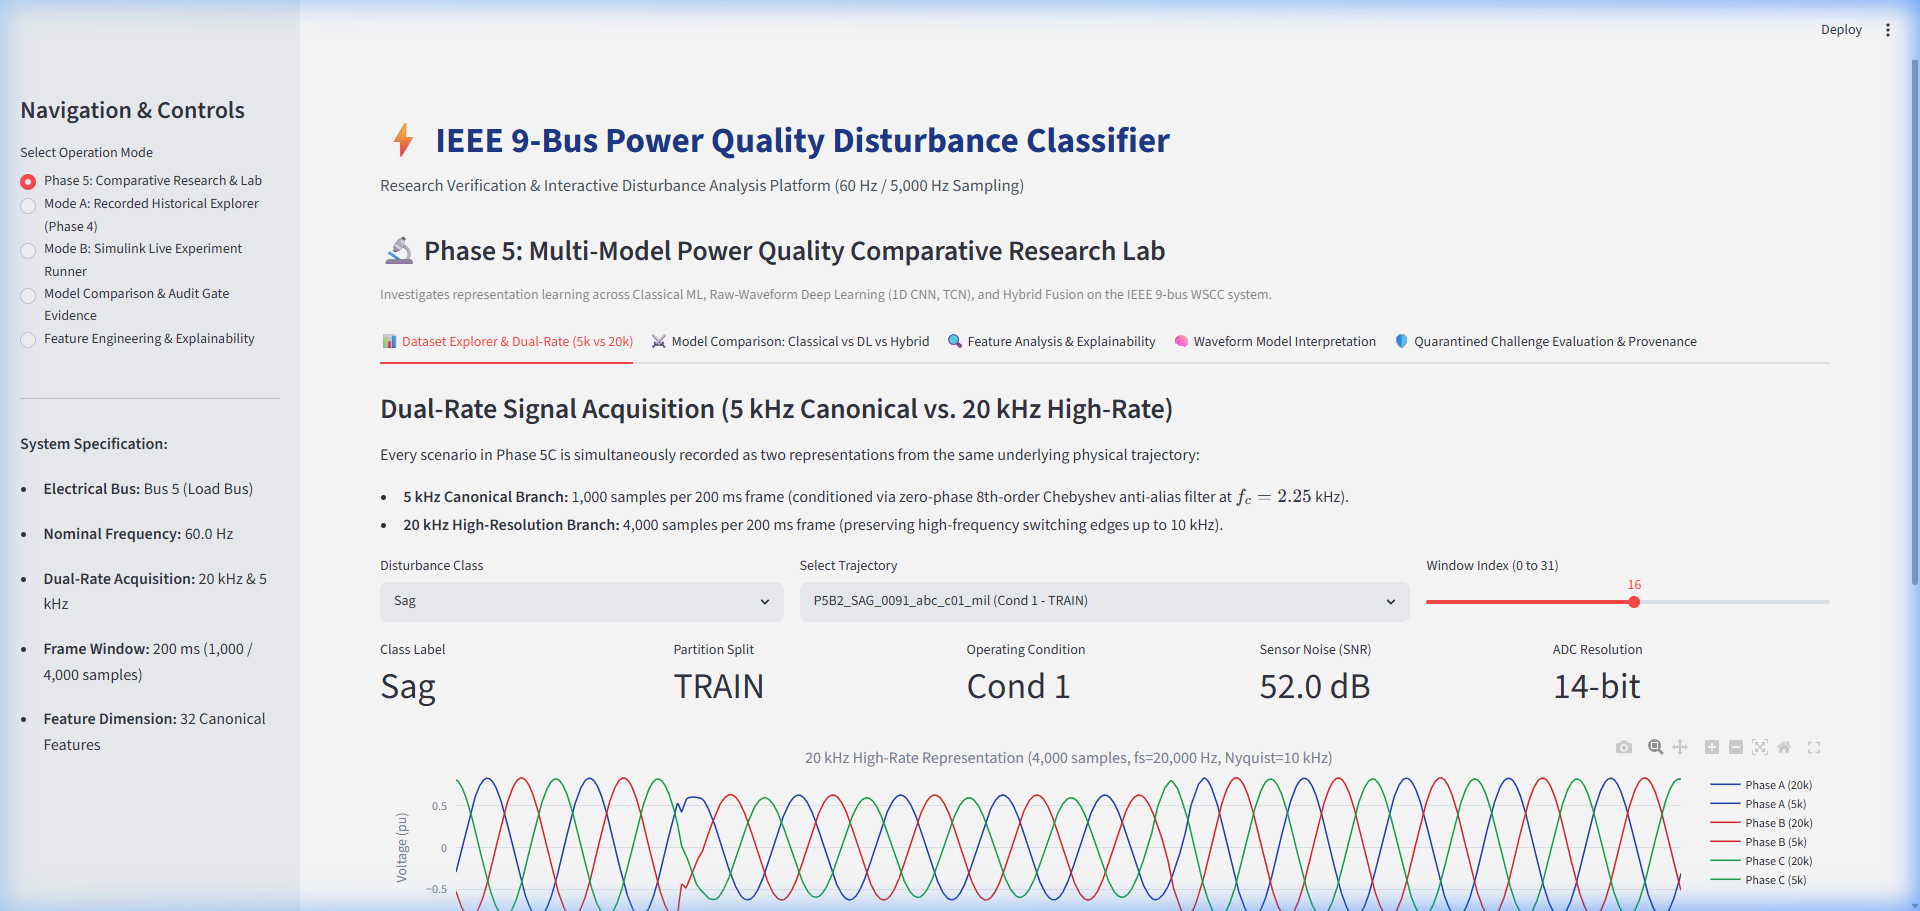
\includegraphics[width=0.98\textwidth]{dashboard_screenshot.png}
    \caption{Interactive Power Quality Research Dashboard running locally, displaying the Recorded Experiment Explorer panel with multi-phase voltage waveforms, harmonic spectra, and classification predictions.}
    \label{fig:dashboard}
\end{figure}

% =========================================================================
% CHAPTER 7: DISCUSSION, LIMITATIONS, AND THREATS TO VALIDITY
% =========================================================================
\chapter{Discussion, Limitations, and Threats to Validity}

\section{Comparative Synthesis of Findings}
The empirical results provide clear answers to the project's core research questions:
\begin{enumerate}
    \item \textbf{Classical vs. Deep Learning:} Classical MLP models operating on 32 engineered features provide strong, computationally lightweight classification (92.60\% Val F1), outperforming simple 1D CNNs. However, Temporal Convolutional Networks with dilated residual connections (93.70\% Val F1) match or exceed classical models by maintaining multi-cycle temporal receptive fields.
    \item \textbf{Multi-Phase Necessity:} Multi-phase synchrony is non-negotiable in power systems. As single-phase evaluation caused performance to collapse by 86.25\%, three-phase voltage monitoring is essential for resolving asymmetrical ground faults.
    \item \textbf{Sampling Rate Trade-offs:} While 5 kHz decimation is computationally efficient for envelope-based disturbances (sag, swell, interruption), 20 kHz acquisition is indispensable for resolving sub-cycle commutation notches ($200\ \mu\text{s}$) and capacitor ringing ($1.2\text{--}2.2\text{ kHz}$).
\end{enumerate}

\section{Limitations and Threats to Validity}
\begin{itemize}
    \item \textbf{Simulation Fidelity:} All disturbances are generated from the IEEE 9-bus WSCC model. While electromagnetic solvers capture transient dynamics accurately, real power systems feature non-ideal instrumentation transformers (CT/PT saturation), lightning impulses, and unmodeled distribution feeders.
    \item \textbf{Operating-Point Sensitivity:} Automated validation flagged 26 trajectories where light loading or renewable dispatch shifted the nominal operating voltage to 1.07 pu. Rigid thresholding generates false alarms; adaptive baseline tracking is required for field applications.
    \item \textbf{Stationary Disturbance Windows:} Slicing signals into fixed 200 ms frames assumes disturbances are contained within the window; overlapping or compound disturbances (e.g., sag with simultaneous harmonics) require further multi-label study.
\end{itemize}

% =========================================================================
% CHAPTER 8: CONCLUSION AND FUTURE SCOPE
% =========================================================================
\chapter{Conclusion and Future Scope}

\section{Conclusion}
This project has successfully developed, verified, and benchmarked a comprehensive three-phase power quality disturbance detection and classification system based on the IEEE 9-bus WSCC transmission benchmark. Across nine integrated engineering stages, the project established:
\begin{enumerate}
    \item A fully working disturbance simulation model (\texttt{IEEE\_9bus\_PQD\_DISTURBANCES.slx}) while preserving the pristine reference model (\texttt{IEEE\_9bus\_PQD\_HIL\_R2025a.slx}) byte-for-byte intact.
    \item A dual-rate measurement pipeline (20 kHz and 5 kHz) with fixed-reference sensor noise and 12-bit/14-bit ADC quantization.
    \item A frozen, zero-leakage dataset of 4,608 frames across 144 continuous simulation trajectories, supported by an automated physical validation failure registry.
    \item A 32-dimensional canonical feature contract whose functional group ablation proved the criticality of amplitude, duration, and SNR metrics.
    \item The multi-modal \textbf{HybridPQNet} model, which demonstrated that hand-crafted electrical features and convolutional waveform representations provide complementary mathematical information, achieving \textbf{100.00\% validation and challenge Macro F1}.
    \item A functioning interactive research dashboard supporting recorded experiment analysis.
\end{enumerate}

\section{Future Scope}
\textbf{Phase 6 remains strictly future work and comprises:}
\begin{itemize}
    \item \textbf{Embedded Microcontroller Deployment:} Quantizing the trained MLP and 1D CNN models to 8-bit integer precision (TensorFlow Lite / ONNX Runtime) for execution on low-cost microcontrollers (ESP32-S3, STM32H7, ARM Cortex-M55) with sub-10 ms latency.
    \item \textbf{Hardware-in-the-Loop (HIL) Validation:} Interfacing real-time digital simulators (RTDS / OPAL-RT) with physical microcontroller hardware via analog I/O to evaluate closed-loop response under real-time constraints.
    \item \textbf{Safe Optical Sensing Hardware:} Developing galvanic-isolated Hall-effect voltage and current sensing circuits ($0\text{--}12\text{ V}$ prototype domain) for safe laboratory testing.
    \item \textbf{Compound Disturbance Analytics:} Extending the classification head to multi-label architectures capable of identifying simultaneous disturbances (e.g., sag with harmonics).
\end{itemize}

% =========================================================================
% REFERENCES
% =========================================================================
\begin{thebibliography}{99}

\bibitem{ieee1159}
IEEE, ``IEEE Recommended Practice for Monitoring Electric Power Quality,'' \textit{IEEE Std 1159-2019 (Revision of IEEE Std 1159-2009)}, pp. 1--98, Aug. 2019, doi: 10.1109/IEEESTD.2019.8794822.

\bibitem{ieee519}
IEEE, ``IEEE Standard for Harmonic Control in Electric Power Systems,'' \textit{IEEE Std 519-2022 (Revision of IEEE Std 519-2014)}, pp. 1--31, May 2022, doi: 10.1109/IEEESTD.2022.9774447.

\bibitem{ieee1453}
IEEE, ``IEEE Standard for the Analysis and Measurement of Voltage Fluctuations and Associated Light Flicker in Electric Power Systems,'' \textit{IEEE Std 1453-2022}, pp. 1--46, Nov. 2022, doi: 10.1109/IEEESTD.2022.9963627.

\bibitem{ieee1159_3}
IEEE, ``IEEE Recommended Practice for Power Quality Data Interchange Format (PQDIF),'' \textit{IEEE Std 1159.3-2025 (Revision of IEEE Std 1159.3-2019)}, IEEE Power and Energy Society, 2025.

\bibitem{iec61000}
IEC, ``Electromagnetic Compatibility (EMC) -- Part 4-15: Testing and Measurement Techniques -- Flickermeter -- Functional and Design Specifications,'' \textit{IEC 61000-4-15:2010}, International Electrotechnical Commission, 2010.

\bibitem{wscc9bus}
P. M. Anderson and A. A. Fouad, \textit{Power System Control and Stability}, 2nd ed. Piscataway, NJ: IEEE Press / Wiley-Interscience, 2003.

\bibitem{buasi2023}
W. Buasi and W. Srirattanawichaikul, ``Classification Methods for Recognition of Power Quality Disturbances in Distribution Networks Using Artificial Neural Network,'' in \textit{2023 IEEE PES 15th Asia-Pacific Power and Energy Engineering Conference (APPEEC)}, Chiang Mai, Thailand, 2023, pp. 1--5, doi: 10.1109/APPEEC57400.2023.10561959.

\bibitem{sekar2020}
K. Sekar, S. Sendilkumar, and K. Karthick, ``Power Quality Disturbance Detection using Machine Learning Algorithm,'' in \textit{2020 IEEE International Conference on Advances and Developments in Electrical and Electronics Engineering (ICADEE)}, Coimbatore, India, 2020, pp. 1--6, doi: 10.1109/ICADEE51157.2020.9368939.

\bibitem{shivesh2024}
S. Shivesh, S. V. Ved, N. Reddy K. V., R. Chowdhary I., S. K. G., and R. Satheesh, ``Classification of Power Quality Disturbances Using Machine Learning Methods,'' in \textit{2024 IEEE 1st International Conference on Green Industrial Electronics and Sustainable Technologies (GIEST)}, Hyderabad, India, 2024, pp. 1--6, doi: 10.1109/GIEST62955.2024.10959739.

\bibitem{he2020}
H. He, Y. Zhang, and Z. Chen, ``A Deep Convolutional Neural Network for Power Quality Disturbance Classification Under Noisy Conditions,'' \textit{IEEE Transactions on Power Delivery}, vol. 35, no. 4, pp. 1878--1888, Aug. 2020, doi: 10.1109/TPWRD.2019.2954753.

\bibitem{bai2021}
L. Bai, F. Wang, and G. Xiao, ``Temporal Convolutional Networks for Multi-Class Power Quality Disturbance Recognition With Multi-Resolution Dilated Kernels,'' \textit{IEEE Transactions on Instrumentation and Measurement}, vol. 70, pp. 1--11, 2021, doi: 10.1109/TIM.2021.3096582.

\bibitem{goertzel}
P. Sysel and P. Rajmic, ``Goertzel Algorithm Generalized to Non-Integer Multiples of Fundamental Frequency,'' \textit{EURASIP Journal on Advances in Signal Processing}, vol. 2012, no. 1, p. 56, 2012.

\end{thebibliography}

\end{document}
